\documentclass[12pt,a4paper]{article}

% =========================
% PAQUETES
% =========================
\usepackage[utf8]{inputenc}
\usepackage[T1]{fontenc}
\usepackage[spanish]{babel}
\usepackage{geometry}
\usepackage{graphicx}
\usepackage{amsmath}
\usepackage{placeins}

\geometry{
    top=2.5cm,
    bottom=2.5cm,
    left=3cm,
    right=3cm
}

\begin{document}

% =========================
% PORTADA
% =========================
\begin{titlepage}
    \centering

    \vspace*{2cm}

    {\Large \textbf{Procesamiento de Señales e Imágenes Biomédicas 16.63}}\\[0.4cm]

    \vspace{3cm}

    {\Huge \textbf{Laboratorio de Adquisición}}\\[0.4cm]
    {\Huge \textbf{de Señales Biomédicas}}\\

    \vspace{3cm}

    {\large
    \textbf{Alumnos}\\[0.8cm]

    Garaguso Fernandez, Facundo -- 65436\\[0.4cm]
    Basualdo, Joaquin -- 65658\\[0.4cm]
    Estrada, Bautista -- 65583
    }

    \vfill

    {\large
    \textbf{Fecha de entrega:} A definir
    }

    \vspace{1.5cm}

\end{titlepage}

% =========================
% RESOLUCIÓN DEL INFORME
% =========================

\clearpage

\section{Formato de registro de la señal de ECG}

En este experimento, las señales de ECG fueron almacenadas en archivos de tipo
\textit{CSV} (\textit{Comma-Separated Values}). Este formato permite representar
datos en forma tabular mediante un archivo de texto plano, por lo que resulta
simple de almacenar, visualizar e importar posteriormente en programas de
procesamiento como Python, MATLAB o Excel.

En particular, los archivos obtenidos en el laboratorio contienen una única
columna denominada \texttt{Sample}, en la cual cada fila corresponde a una
muestra consecutiva de la señal adquirida. Los archivos no contienen una columna
de tiempo ni almacenan explícitamente la frecuencia de muestreo, por lo que la
información temporal debe reconstruirse a partir de la frecuencia de adquisición.

Si se conoce la frecuencia de muestreo $f_s$, el instante correspondiente a la
muestra $n$ puede determinarse como

\[
t[n] = \frac{n}{f_s}
\]

El formato CSV resulta adecuado para este trabajo debido a su simplicidad y a que
permite acceder directamente a las muestras para realizar posteriormente el
acondicionamiento de la señal, la detección de los complejos QRS y el análisis de
la frecuencia cardíaca.

Sin embargo, existen otros formatos utilizados para almacenar señales
electrocardiográficas. Entre los principales se encuentran:

\begin{itemize}
    \item \textbf{WFDB (\textit{WaveForm DataBase}):} formato ampliamente
    utilizado en bases de datos de señales fisiológicas como PhysioNet. Un
    registro suele estar compuesto por un archivo de cabecera \texttt{.hea}, que
    contiene información como la frecuencia de muestreo, cantidad de señales,
    unidades y calibración, y uno o más archivos con las muestras de las señales,
    habitualmente \texttt{.dat}. También permite incorporar archivos de
    anotaciones para indicar eventos como complejos QRS o tipos de latidos.

    \item \textbf{EDF/EDF+ (\textit{European Data Format}):} formato diseñado
    específicamente para almacenar señales biomédicas. Permite guardar múltiples
    canales dentro de un mismo archivo junto con información de calibración,
    cantidad de muestras y características de cada señal. La extensión EDF+
    permite además incorporar anotaciones.

    \item \textbf{DICOM:} estándar utilizado principalmente para el intercambio
    y almacenamiento de información médica dentro de sistemas clínicos. Además
    de imágenes médicas, DICOM contempla objetos específicos para almacenar
    formas de onda fisiológicas, incluyendo registros electrocardiográficos.

    \item \textbf{HL7 aECG (\textit{Annotated ECG}):} formato basado en XML que
    permite almacenar tanto la señal electrocardiográfica como información y
    anotaciones asociadas al registro. Es utilizado especialmente para el
    intercambio estandarizado de ECG digitales y en determinados contextos
    regulatorios y de investigación clínica.
\end{itemize}

A diferencia de estos formatos especializados, el archivo CSV utilizado en el
laboratorio contiene esencialmente las muestras de la señal y no incorpora de
forma estructurada metadatos clínicos, información de calibración, derivaciones,
frecuencia de muestreo o anotaciones. Por este motivo, estos parámetros deben
conocerse a partir de las condiciones con las que se realizó la adquisición.


\section{Frecuencia de muestreo}

La frecuencia de muestreo $f_s$ indica la cantidad de muestras adquiridas por
unidad de tiempo y puede calcularse como

\[
f_s = \frac{N}{T}
\]

donde $N$ es el número total de muestras adquiridas y $T$ es la duración del
registro expresada en segundos.

Para el registro realizado en reposo, el archivo \texttt{ecg\_data\_pre.csv}
contiene un total de

\[
N_{\mathrm{pre}} = 28800
\]

muestras. De acuerdo con el procedimiento experimental, el registro en reposo
tuvo una duración de un minuto, es decir,

\[
T_{\mathrm{pre}} = 60~\mathrm{s}
\]

Por lo tanto,

\[
f_s =
\frac{28800}{60~\mathrm{s}}
=
480~\mathrm{Hz}
\]

Esto significa que el sistema adquirió nominalmente \textbf{480 muestras por
segundo}. El intervalo temporal entre dos muestras consecutivas es, entonces,

\[
T_s = \frac{1}{f_s}
     = \frac{1}{480}
     \approx 2.083~\mathrm{ms}
\]

El segundo registro permite verificar la consistencia de este resultado. El
archivo \texttt{ecg\_data\_post.csv}, correspondiente al período posterior a la
actividad física, contiene

\[
N_{\mathrm{post}} = 86600
\]

muestras. Considerando la misma frecuencia de muestreo,

\[
T_{\mathrm{post}}
=
\frac{86600}{480}
\approx
180.42~\mathrm{s}
\]

lo cual equivale aproximadamente a

\[
T_{\mathrm{post}} \approx 3.01~\mathrm{min}
\]

Este resultado coincide con el procedimiento experimental, en el cual se debía
registrar aproximadamente tres minutos de ECG luego de la actividad física.

En consecuencia, se determina que la señal de ECG fue registrada con una
\textbf{frecuencia de muestreo nominal de}

\[
 \boxed{f_s = 480~\mathrm{Hz}}
\]

Dado que los archivos CSV no incluyen una columna temporal ni almacenan
explícitamente el valor de $f_s$, esta frecuencia se determinó a partir del
número de muestras y de la duración conocida de los registros.

% =========================
% INCISO 3
% =========================

\section{Sistema de adquisición y derivaciones electrocardiográficas}

\subsection{Resolución de la placa AD8232}

La placa AD8232 utilizada para la adquisición de la señal no realiza por sí
misma la conversión analógico-digital de la señal de ECG. El AD8232 es un
\textit{front-end} analógico diseñado específicamente para el
acondicionamiento de biopotenciales cardíacos. Su función consiste en recibir
las pequeñas diferencias de potencial provenientes de los electrodos,
amplificarlas y filtrarlas para obtener una señal adecuada para su posterior
digitalización (Analog Devices, 2020).

\begin{figure}[htbp]
    \centering
    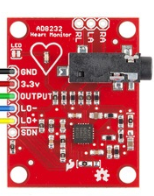
\includegraphics[width=0.55\textwidth]{Imagenes/AD8232.png}
    \caption{Placa AD8232 utilizada para la adquisición y acondicionamiento de la señal de ECG.}
    \label{fig:ad8232}
\end{figure}

Entre sus principales características se encuentra un amplificador de
instrumentación con una ganancia nominal de

\[
G = 100
\]

además de la posibilidad de implementar filtrado pasa-altos y pasa-bajos y un
circuito de \textit{Right Leg Drive} (RLD) para mejorar el rechazo de señales
de modo común.

Por este motivo, no es correcto asignar al AD8232 una resolución de, por
ejemplo, 10, 12 o 16 bits. La resolución digital del registro queda determinada
por el conversor analógico-digital (ADC) del microcontrolador conectado a la
salida del AD8232 y por la configuración utilizada durante la adquisición.

En términos generales, para un ADC de $N$ bits existen

\[
2^N
\]

niveles digitales posibles. Si el rango de entrada del conversor está
determinado por una tensión de referencia $V_{\mathrm{ref}}$, la resolución
ideal en tensión puede expresarse como

\[
\Delta V = \frac{V_{\mathrm{ref}}}{2^N}
\]

En consecuencia, debe distinguirse entre el \textbf{acondicionamiento
analógico}, realizado por el AD8232, y la \textbf{resolución de
digitalización}, determinada por el ADC utilizado posteriormente. El AD8232
entrega una señal analógica acondicionada y, por lo tanto, no posee una
resolución digital propia expresable en bits.


\subsection{Utilización de electrodos en los miembros}

En un electrocardiograma clínico convencional se utilizan electrodos ubicados
tanto sobre los miembros como sobre el tórax. A diferencia de una adquisición
simplificada destinada principalmente al seguimiento de la frecuencia
cardíaca, el ECG clínico busca observar la actividad eléctrica del corazón
desde diferentes direcciones espaciales.

Los electrodos ubicados en los miembros permiten obtener las derivaciones
correspondientes al \textbf{plano frontal} del corazón. A partir de los
electrodos colocados en el brazo derecho, brazo izquierdo y miembro inferior
izquierdo pueden obtenerse las tres derivaciones bipolares de Einthoven:

\[
\mathrm{I} = V_{\mathrm{LA}} - V_{\mathrm{RA}}
\]

\[
\mathrm{II} = V_{\mathrm{LL}} - V_{\mathrm{RA}}
\]

\[
\mathrm{III} = V_{\mathrm{LL}} - V_{\mathrm{LA}}
\]

donde RA corresponde al brazo derecho, LA al brazo izquierdo y LL a la pierna izquierda.

A partir de estos mismos electrodos también se construyen las derivaciones
unipolares aumentadas

\[
aVR \qquad aVL \qquad aVF
\]

En conjunto, las derivaciones I, II, III, aVR, aVL y aVF permiten observar la
propagación de la actividad eléctrica cardíaca desde seis orientaciones
diferentes dentro del plano frontal (Ashley \& Niebauer, 2004; Noble et al.,
1990).

\begin{figure}[htbp]
    \centering
    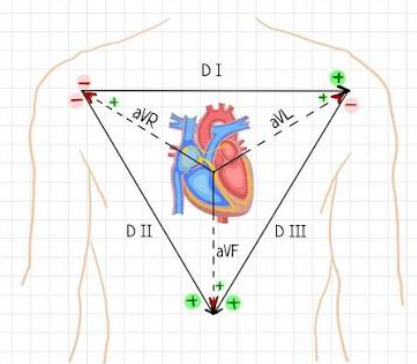
\includegraphics[width=0.70\textwidth]{Imagenes/PlanoFrontal.png}
    \caption{Derivaciones electrocardiográficas correspondientes al plano frontal: I, II, III, aVR, aVL y aVF.}
    \label{fig:plano-frontal}
\end{figure}

El electrodo colocado habitualmente en el miembro inferior derecho cumple una
función diferente. No genera por sí mismo una nueva derivación clínica, sino
que suele emplearse como electrodo de referencia o como electrodo conducido
para reducir la interferencia de modo común. El AD8232 incorpora precisamente
un amplificador de \textit{Right Leg Drive}, cuya salida puede conectarse a un
electrodo de referencia con el objetivo de mejorar el rechazo de interferencias
comunes presentes sobre el paciente (Analog Devices, 2020).

Por lo tanto, la utilización de electrodos en los miembros no tiene únicamente
como objetivo obtener una señal cardíaca de mayor amplitud, sino principalmente
observar el vector eléctrico cardíaco desde diferentes direcciones.
Esto aporta información que una única derivación no puede proporcionar.


\subsection{Otras derivaciones electrocardiográficas e información espacial}

Un ECG clínico estándar utiliza diez electrodos físicos para obtener
doce derivaciones. Estas doce derivaciones no corresponden a doce
electrodos independientes, sino a diferentes combinaciones de los potenciales
registrados por los electrodos ubicados sobre los miembros y el tórax.

Las derivaciones pueden agruparse de la siguiente manera:

\begin{center}
\begin{tabular}{|p{3.5cm}|p{4cm}|p{5cm}|}
\hline
\textbf{Grupo} & \textbf{Derivaciones} & \textbf{Plano observado} \\
\hline
Bipolares de miembros &
I, II, III &
Plano frontal \\
\hline
Aumentadas de miembros &
aVR, aVL, aVF &
Plano frontal \\
\hline
Precordiales &
V1, V2, V3, V4, V5, V6 &
Plano horizontal o transversal \\
\hline
\end{tabular}
\end{center}

Las derivaciones de los miembros permiten analizar la actividad eléctrica en
el plano frontal, mientras que las derivaciones precordiales V1 a V6 permiten
observar el corazón desde diferentes posiciones en el plano horizontal
(Ashley \& Niebauer, 2004).

\begin{figure}[htbp]
    \centering
    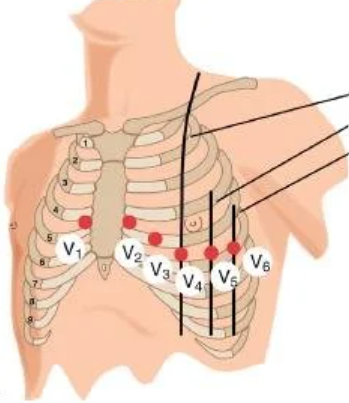
\includegraphics[width=0.70\textwidth]{Imagenes/PlanoHorizontal.png}
    \caption{Ubicación de las derivaciones precordiales V1 a V6 y representación del plano horizontal del corazón.}
    \label{fig:plano-horizontal}
\end{figure}

De manera aproximada, determinadas derivaciones presentan una mayor
sensibilidad a la actividad eléctrica de ciertas regiones cardíacas:

\begin{itemize}
    \item \textbf{Región inferior:} II, III y aVF.
    \item \textbf{Región lateral:} I, aVL, V5 y V6.
    \item \textbf{Región septal:} V1 y V2.
    \item \textbf{Región anterior:} V3 y V4.
\end{itemize}

Cada derivación registra la proyección del vector eléctrico cardíaco sobre un
eje diferente. Una onda de despolarización que se dirige hacia el electrodo
positivo produce una deflexión predominantemente positiva, mientras que una
onda que se aleja de este produce una deflexión predominantemente negativa.
Por este motivo, una misma activación cardíaca presenta morfologías diferentes
según la derivación desde la cual sea observada (Noble et al., 1990).

La disponibilidad simultánea de múltiples derivaciones proporciona al
profesional una representación espacial mucho más completa de la actividad
eléctrica cardíaca. Esto permite estudiar, entre otros aspectos, la dirección
del eje eléctrico, la secuencia de despolarización y repolarización, la
propagación de los impulsos a través del sistema de conducción y la presencia
de alteraciones regionales de la actividad eléctrica.

Por ejemplo, una modificación que aparece simultáneamente en un determinado
grupo de derivaciones puede asociarse con una región particular del corazón.
De esta forma, el análisis conjunto de las doce derivaciones puede contribuir
a la identificación y localización de alteraciones de conducción, cambios
compatibles con isquemia o lesión miocárdica, trastornos del ritmo y otras
alteraciones cardíacas. La principal ventaja respecto de una adquisición de
una única derivación es, por lo tanto, la posibilidad de analizar no solamente
la evolución temporal de la señal, sino también la dirección espacial
de la actividad eléctrica cardíaca.

% =========================
% INCISO 4
% =========================

\section{Necesidad de acondicionamiento y preprocesamiento}

Antes de realizar la detección de los complejos QRS y el análisis de la
frecuencia cardíaca es necesario evaluar si las señales adquiridas requieren
algún tipo de acondicionamiento. Una señal de ECG presenta amplitudes pequeñas
y su contenido de interés se encuentra concentrado principalmente en bajas
frecuencias, por lo que puede verse afectada por perturbaciones introducidas
durante el proceso de adquisición.

Para determinar cuáles de estas perturbaciones se encuentran efectivamente
presentes en los registros obtenidos, se analizaron inicialmente las señales
sin aplicar ningún tipo de filtrado. En las Figuras~\ref{fig:ecg-pre-completo}
y~\ref{fig:ecg-post-completo} se presentan los registros completos
correspondientes al estado de reposo y al período posterior a la actividad
física.

\begin{figure}[htbp]
    \centering
    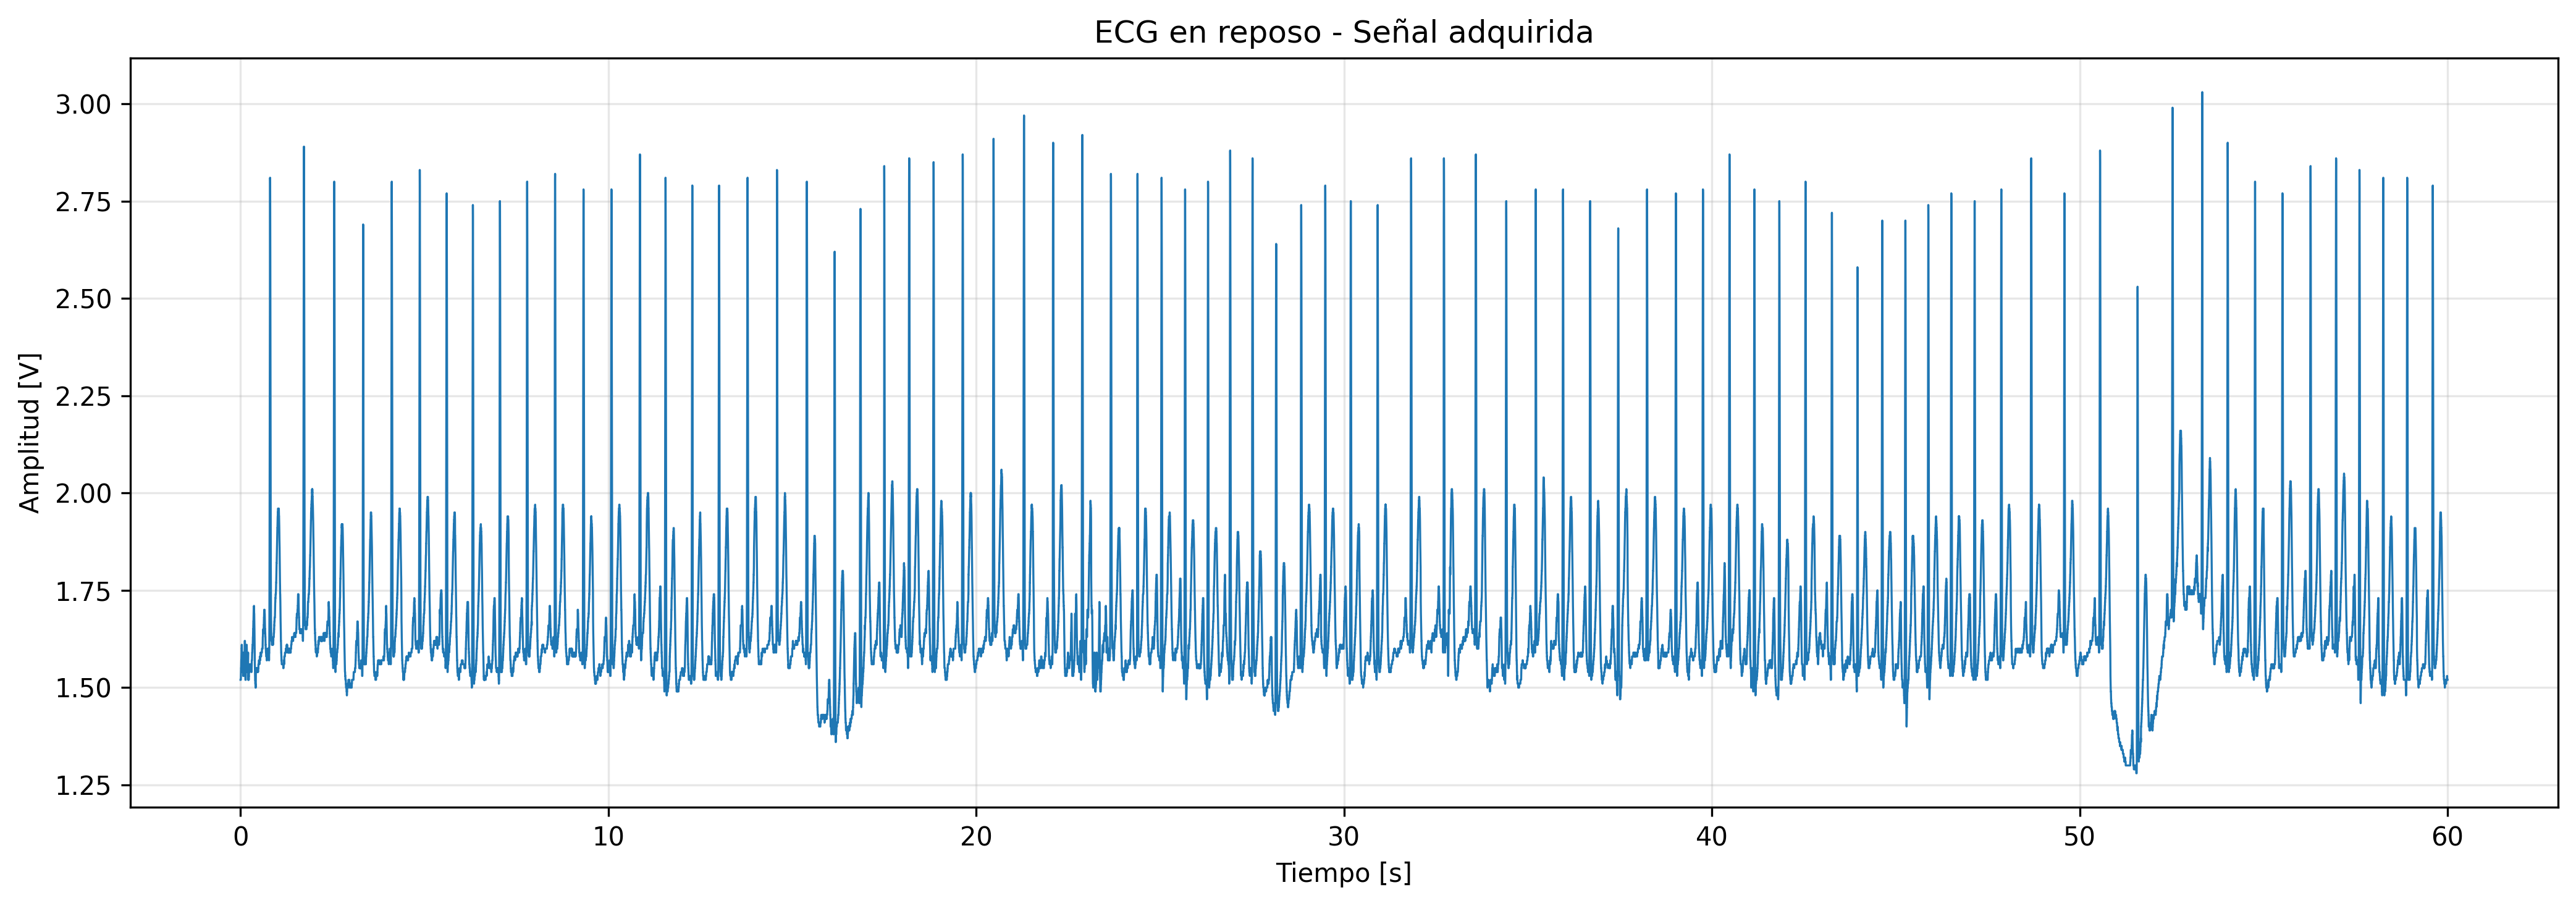
\includegraphics[width=0.95\textwidth]{Imagenes/ECG_Pre_Completo.png}
    \caption{Registro completo de ECG obtenido en reposo}
    \label{fig:ecg-pre-completo}
\end{figure}

\begin{figure}[htbp]
    \centering
    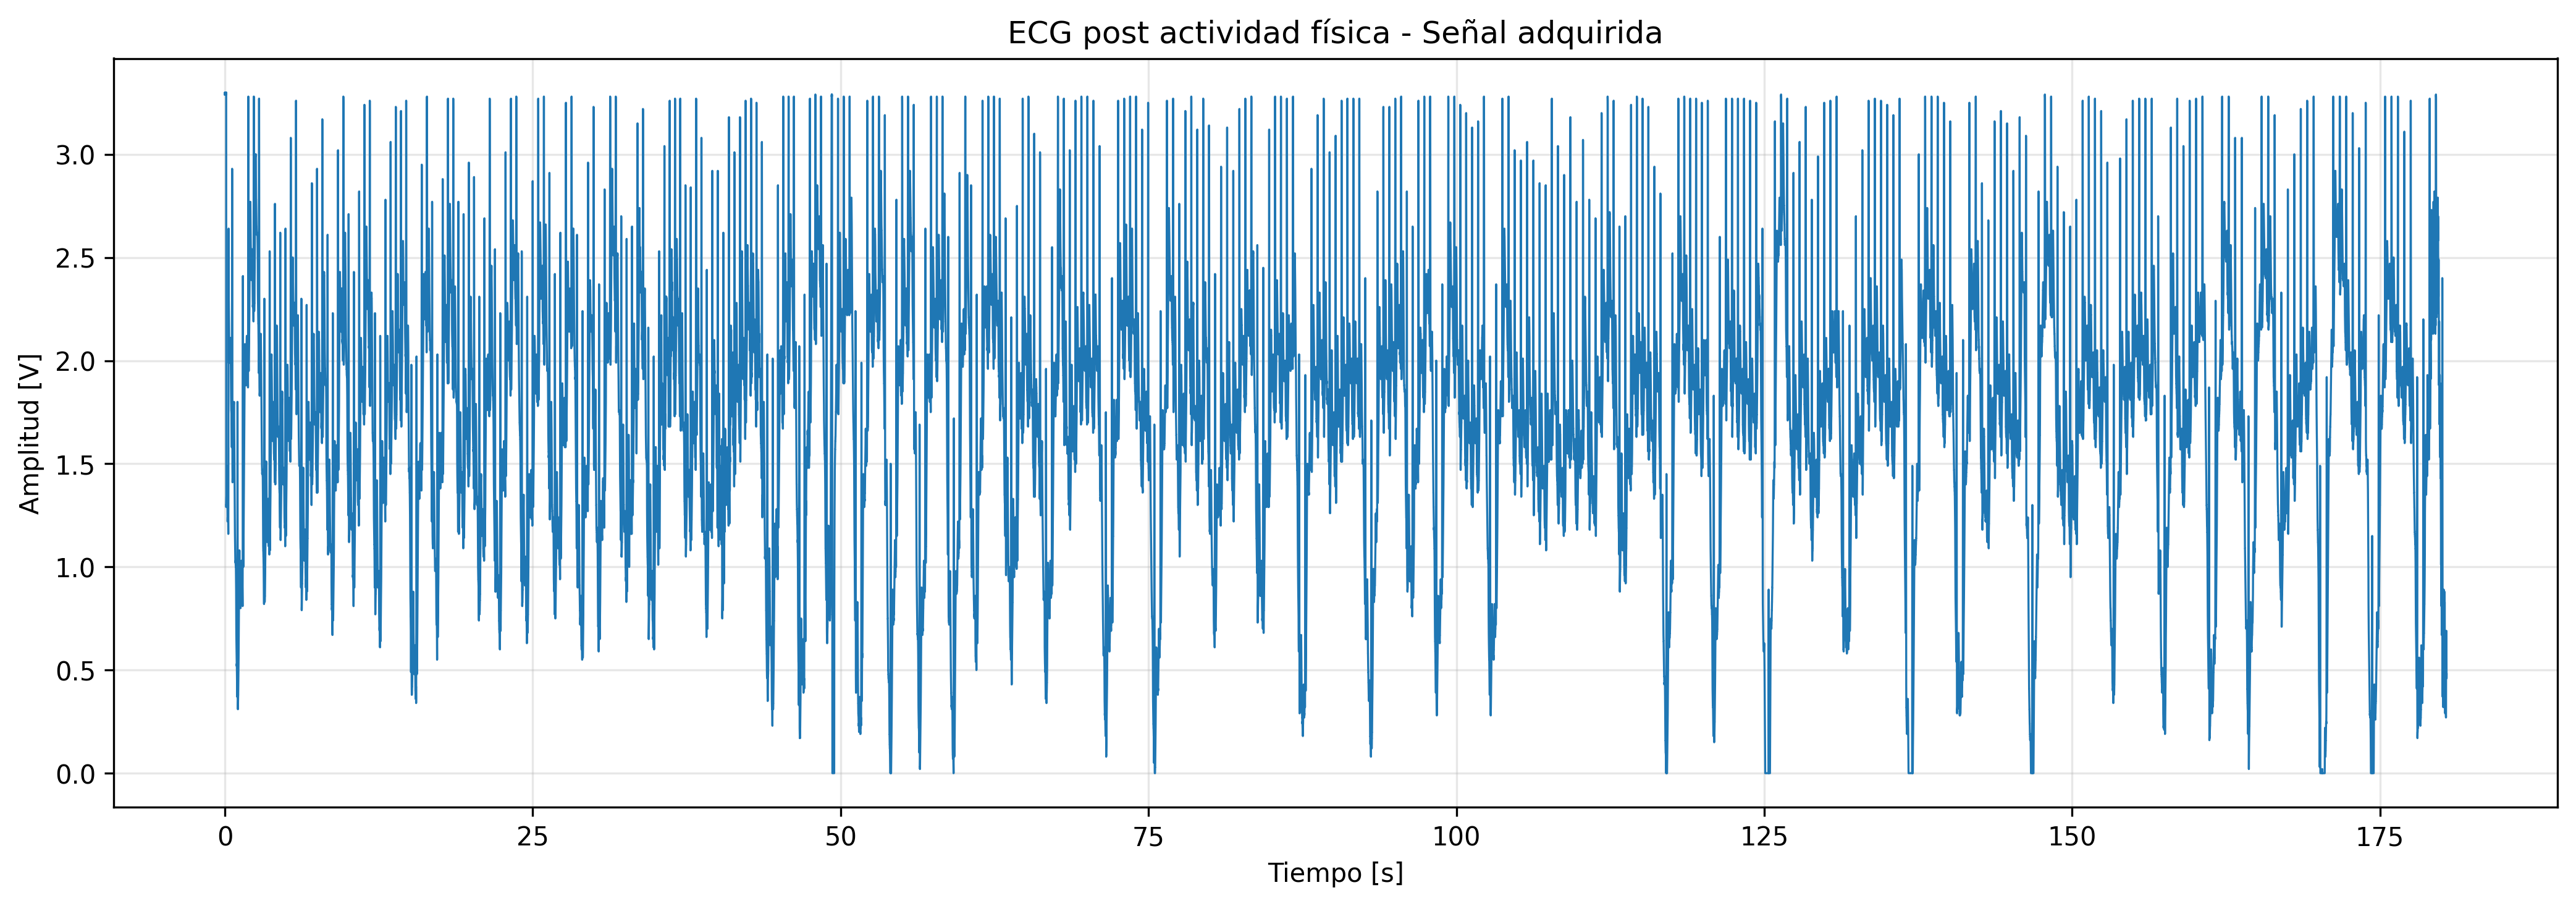
\includegraphics[width=0.95\textwidth]{Imagenes/ECG_Post_Completo.png}
    \caption{Registro completo de ECG obtenido luego de la actividad física}
    \label{fig:ecg-post-completo}
\end{figure}

A partir de estas representaciones puede observarse una diferencia importante
entre ambos registros. La señal obtenida en reposo presenta una línea de base
relativamente estable durante la mayor parte de la adquisición, aunque se
observan algunas variaciones lentas de mayor amplitud en determinados
intervalos. En cambio, en el registro posterior al ejercicio aparecen
variaciones mucho más pronunciadas y sostenidas de la línea de base.

Para analizar con mayor detalle la morfología de las señales se representaron
también ventanas temporales de diez segundos, mostradas en las
Figuras~\ref{fig:ecg-pre-zoom} y~\ref{fig:ecg-post-zoom}.

\begin{figure}[htbp]
    \centering
    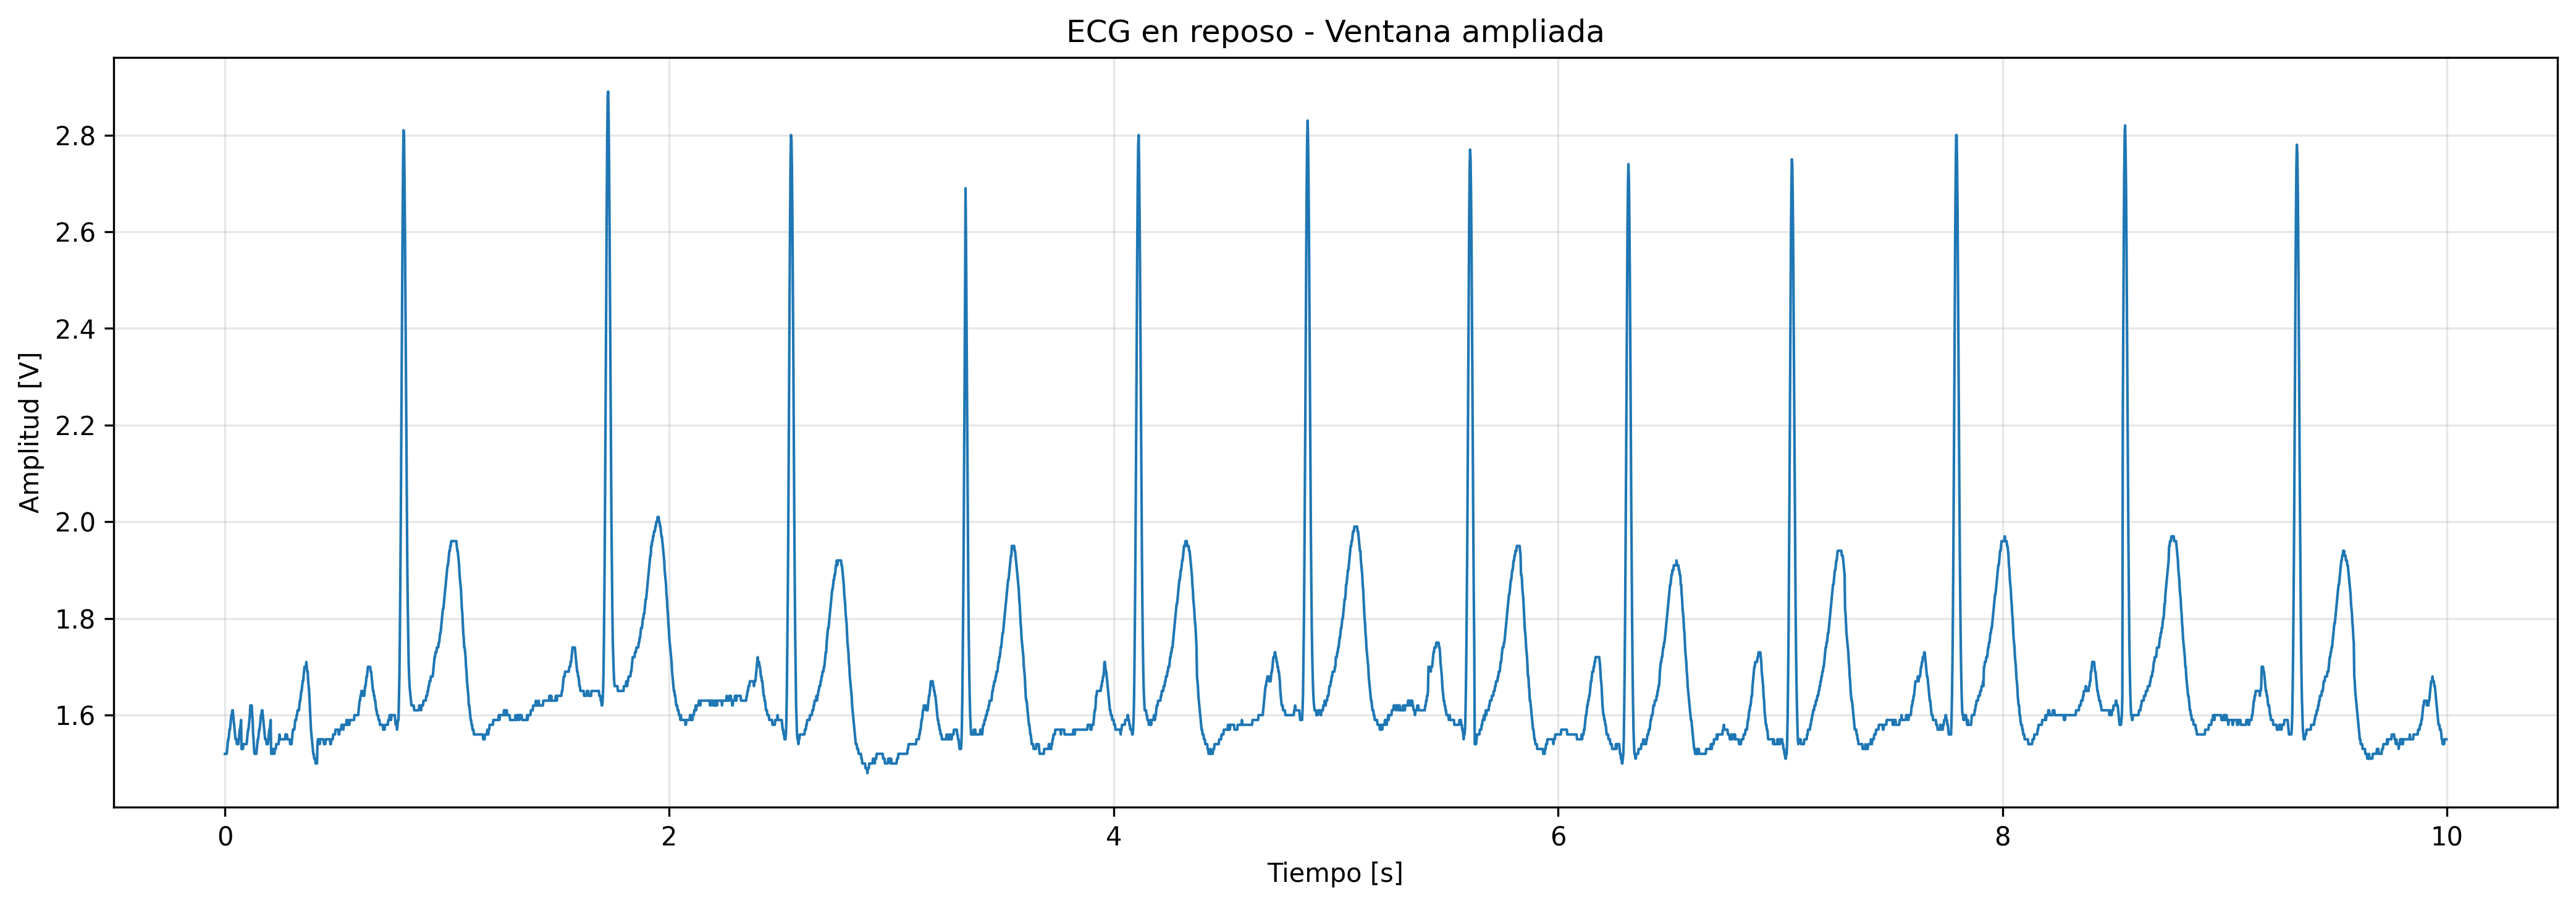
\includegraphics[width=0.95\textwidth]{Imagenes/ECG_Pre_Zoom.png}
    \caption{Ventana ampliada de diez segundos del ECG registrado en reposo}
    \label{fig:ecg-pre-zoom}
\end{figure}

\begin{figure}[htbp]
    \centering
    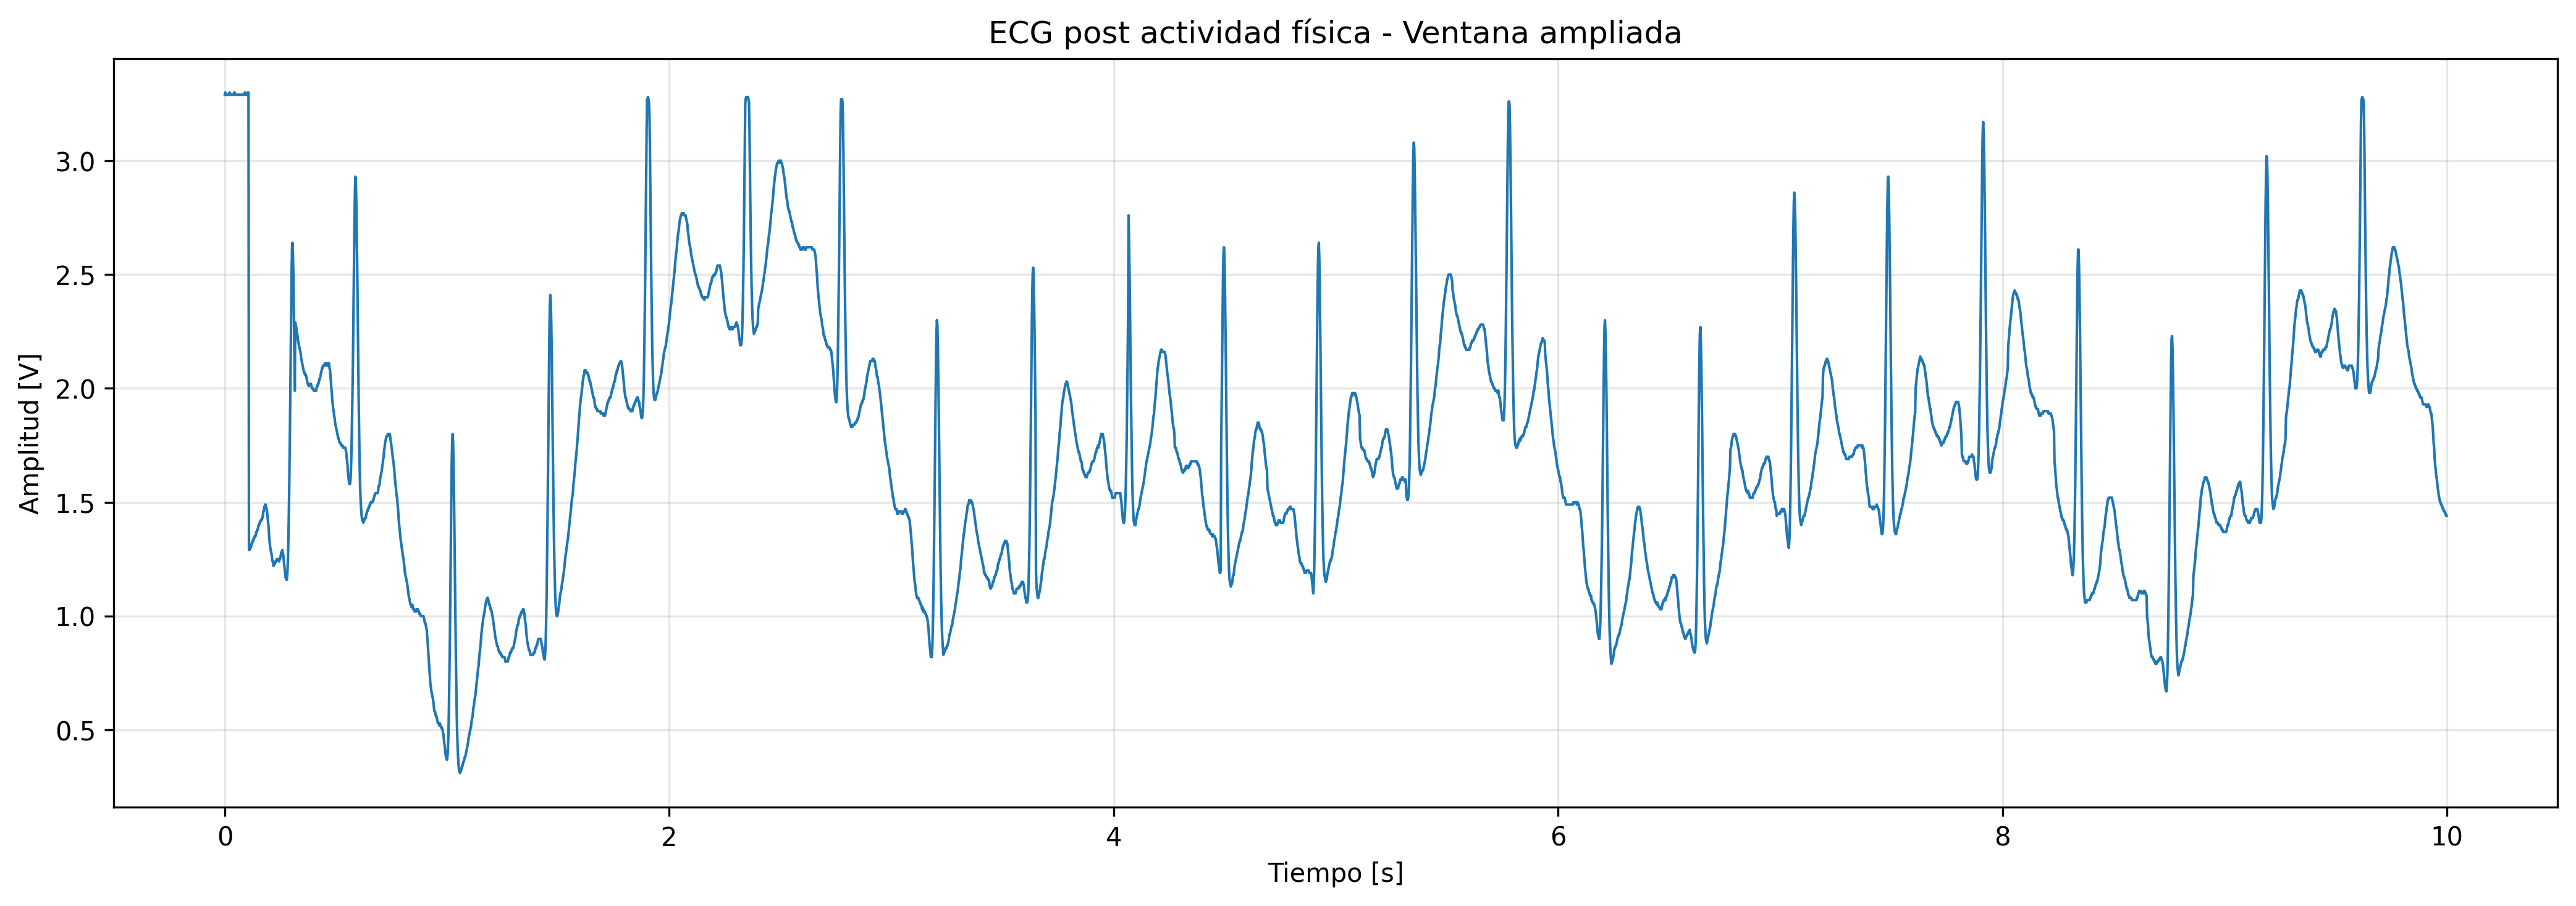
\includegraphics[width=0.95\textwidth]{Imagenes/ECG_Post_Zoom.png}
    \caption{Ventana ampliada de diez segundos del ECG registrado luego de la actividad física}
    \label{fig:ecg-post-zoom}
\end{figure}

\FloatBarrier

\subsection{Componente de continua}

En ambos registros se observa que la señal se encuentra desplazada respecto de
cero. El valor medio calculado para el registro en reposo es aproximadamente
1.67 V, mientras que para el registro posterior a la actividad física es
aproximadamente 1.68 V.

Este desplazamiento no representa una componente fisiológica del ECG, sino que
se encuentra asociado al sistema de adquisición y al nivel de referencia
utilizado para representar una señal bipolar mediante una electrónica
alimentada con tensión positiva.

Por este motivo, antes del procesamiento resulta necesario eliminar esta
componente de continua y centrar la señal respecto de su línea de base.

\subsection{Deriva de la línea de base}

Otro fenómeno claramente observable es la variación lenta de la línea de base.
En el registro en reposo este efecto es relativamente reducido durante la mayor
parte del tiempo, aunque aparecen algunos intervalos donde la señal se desplaza
lentamente respecto de su nivel habitual.

Este fenómeno resulta mucho más evidente en el registro posterior a la actividad
física. Como puede observarse en la Figura~\ref{fig:ecg-post-zoom}, el nivel
alrededor del cual se desarrolla la señal varía considerablemente dentro de una
misma ventana de diez segundos.

Estas variaciones de baja frecuencia son compatibles con una deriva de la línea
de base. Dentro del sistema de adquisición pueden estar relacionadas con
variaciones lentas en la interfaz electrodo-piel y con cambios en las condiciones
de contacto de los electrodos.

La presencia de esta componente puede dificultar la posterior detección
automática de los complejos QRS, ya que modifica continuamente el nivel de
referencia respecto del cual se encuentran los picos.

De acuerdo con el procedimiento de filtrado estudiado, una alternativa para
reducir este fenómeno consiste en aplicar un filtro pasa-altos con una frecuencia
de corte de

\[
f_c = 0.5~\mathrm{Hz}
\]

Para evitar introducir un desplazamiento temporal de los complejos QRS puede
utilizarse un filtro IIR aplicado en forma \textit{forward-backward}.

\subsection{Saturación del sistema de adquisición}

Una característica especialmente relevante del registro posterior a la
actividad física es la presencia de valores que alcanzan los límites del rango
de adquisición.

En este registro se obtuvieron valores mínimos de aproximadamente 0 V y máximos
de aproximadamente 3.3 V. En la Figura~\ref{fig:ecg-post-zoom} puede observarse
incluso, al comienzo del intervalo representado, una región en la cual la señal
permanece momentáneamente próxima al límite superior.

Este comportamiento es compatible con saturación o \textit{clipping} del sistema
de adquisición. Cuando la amplitud de la señal supera el rango que puede
representar el sistema, los valores quedan limitados al máximo o mínimo
disponible y se pierde información sobre la forma real de la señal.

Este efecto es particularmente importante para la posterior detección de
latidos, ya que una transición abrupta asociada a una saturación podría ser
interpretada incorrectamente como un complejo QRS.

A diferencia del ruido aditivo o de la deriva, la información perdida por
saturación no puede recuperarse mediante filtrado digital. Por este motivo,
estos intervalos deberán ser identificados y considerados al momento de aplicar
el algoritmo de detección.

\subsection{Interferencia eléctrica}

Otra fuente de ruido considerada en la adquisición de ECG es la interferencia
eléctrica proveniente de la red y de otros dispositivos presentes en el entorno.
Este tipo de perturbación aparece como una componente aproximadamente periódica
superpuesta a la señal y puede reducirse mediante un filtro
\textit{notch} centrado en la frecuencia interferente.

Sin embargo, a partir de las representaciones temporales de las
Figuras~\ref{fig:ecg-pre-zoom} y~\ref{fig:ecg-post-zoom} no se identifica una
oscilación de alta frecuencia claramente dominante que permita afirmar, por
simple inspección visual, la presencia significativa de ruido de línea.

Por este motivo, no resulta apropiado aplicar directamente un filtro
\textit{notch} únicamente por tratarse de una señal de ECG. Antes de hacerlo
será necesario analizar el contenido frecuencial de los registros y verificar
si efectivamente existe una componente espectral concentrada en la frecuencia
de la red eléctrica.

\subsection{Ruido de alta frecuencia}

En las ventanas ampliadas pueden observarse pequeñas fluctuaciones superpuestas
a la señal, aunque su amplitud resulta considerablemente menor que las
variaciones de baja frecuencia observadas especialmente en el registro
posterior al ejercicio.

Por lo tanto, a partir de la inspección visual no puede considerarse al ruido
de alta frecuencia como la perturbación predominante de estos registros. Su
presencia deberá evaluarse posteriormente mediante el análisis frecuencial antes
de decidir si es necesario incorporar una etapa adicional de filtrado.

\subsection{Conclusión del análisis previo}

A partir de la inspección de las señales adquiridas se concluye que es necesario
realizar un acondicionamiento antes de aplicar el algoritmo de detección de
latidos.

Las principales características encontradas son:

\begin{itemize}
    \item presencia de una componente de continua cercana a 1.67 V
    \item deriva de la línea de base, particularmente importante en el registro
    posterior a la actividad física
    \item presencia de segmentos que alcanzan los límites del rango de
    adquisición en el registro posterior al ejercicio
    \item pequeñas componentes de ruido superpuestas a la señal
    \item ausencia de evidencia visual suficiente para afirmar la presencia de
    una interferencia de línea dominante
\end{itemize}

En consecuencia, el preprocesamiento deberá comenzar por la eliminación de la
componente continua y la atenuación de las variaciones de muy baja frecuencia.
Posteriormente deberá analizarse el contenido espectral de la señal para
determinar si resulta necesaria una etapa específica de rechazo de ruido de
línea.

El objetivo de estas operaciones será mejorar la relación señal-ruido sin
alterar significativamente la localización temporal de los complejos QRS, ya
que esta información será utilizada posteriormente para construir el tacograma
y estudiar la variación de la frecuencia cardíaca.

% =========================
% INCISO 5
% =========================

\section{Acondicionamiento de las señales}

A partir del análisis realizado en el inciso anterior se procedió al
acondicionamiento de ambas señales de ECG. El objetivo de esta etapa fue reducir
las componentes que no resultan de interés para el posterior análisis de la
frecuencia cardíaca, procurando conservar la localización temporal y la
morfología de los complejos QRS.

El procesamiento se realizó de manera progresiva, evaluando el efecto de cada
etapa antes de continuar con la siguiente.

\subsection{Evaluación y eliminación de la componente continua}

Como se observó previamente, ambas señales presentan un desplazamiento respecto
de cero. El valor medio del registro en reposo fue aproximadamente

\[
\overline{x}_{\mathrm{pre}} \approx 1.67~\mathrm{V}
\]

mientras que para el registro posterior a la actividad física se obtuvo

\[
\overline{x}_{\mathrm{post}} \approx 1.68~\mathrm{V}
\]

En las Figuras~\ref{fig:offset-pre} y~\ref{fig:offset-post} se muestran las
señales originales junto con sus respectivos valores medios.

\begin{figure}[htbp]
    \centering
    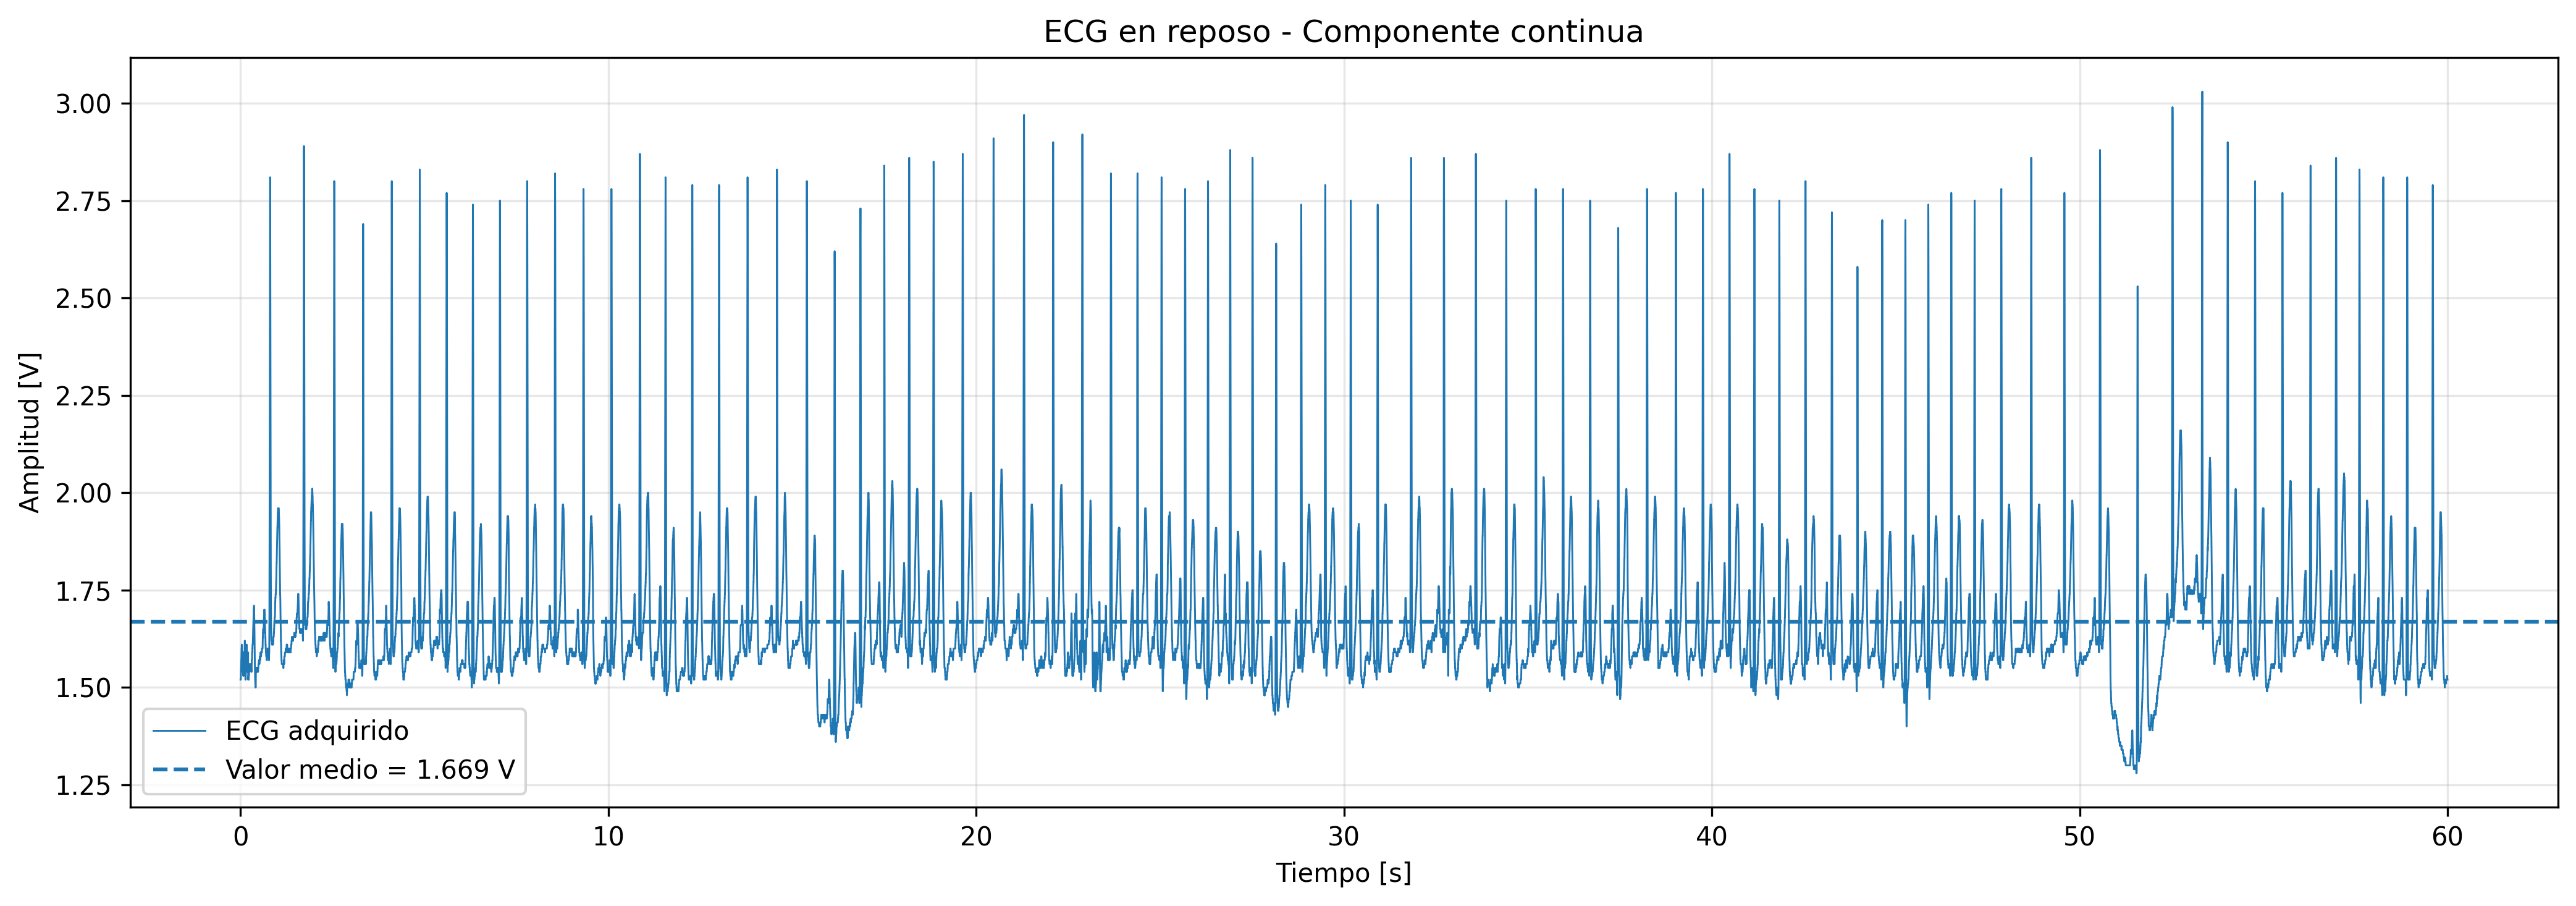
\includegraphics[width=0.95\textwidth]{Imagenes/ECG_Pre_Offset.png}
    \caption{Señal de ECG en reposo y valor medio del registro}
    \label{fig:offset-pre}
\end{figure}

\begin{figure}[htbp]
    \centering
    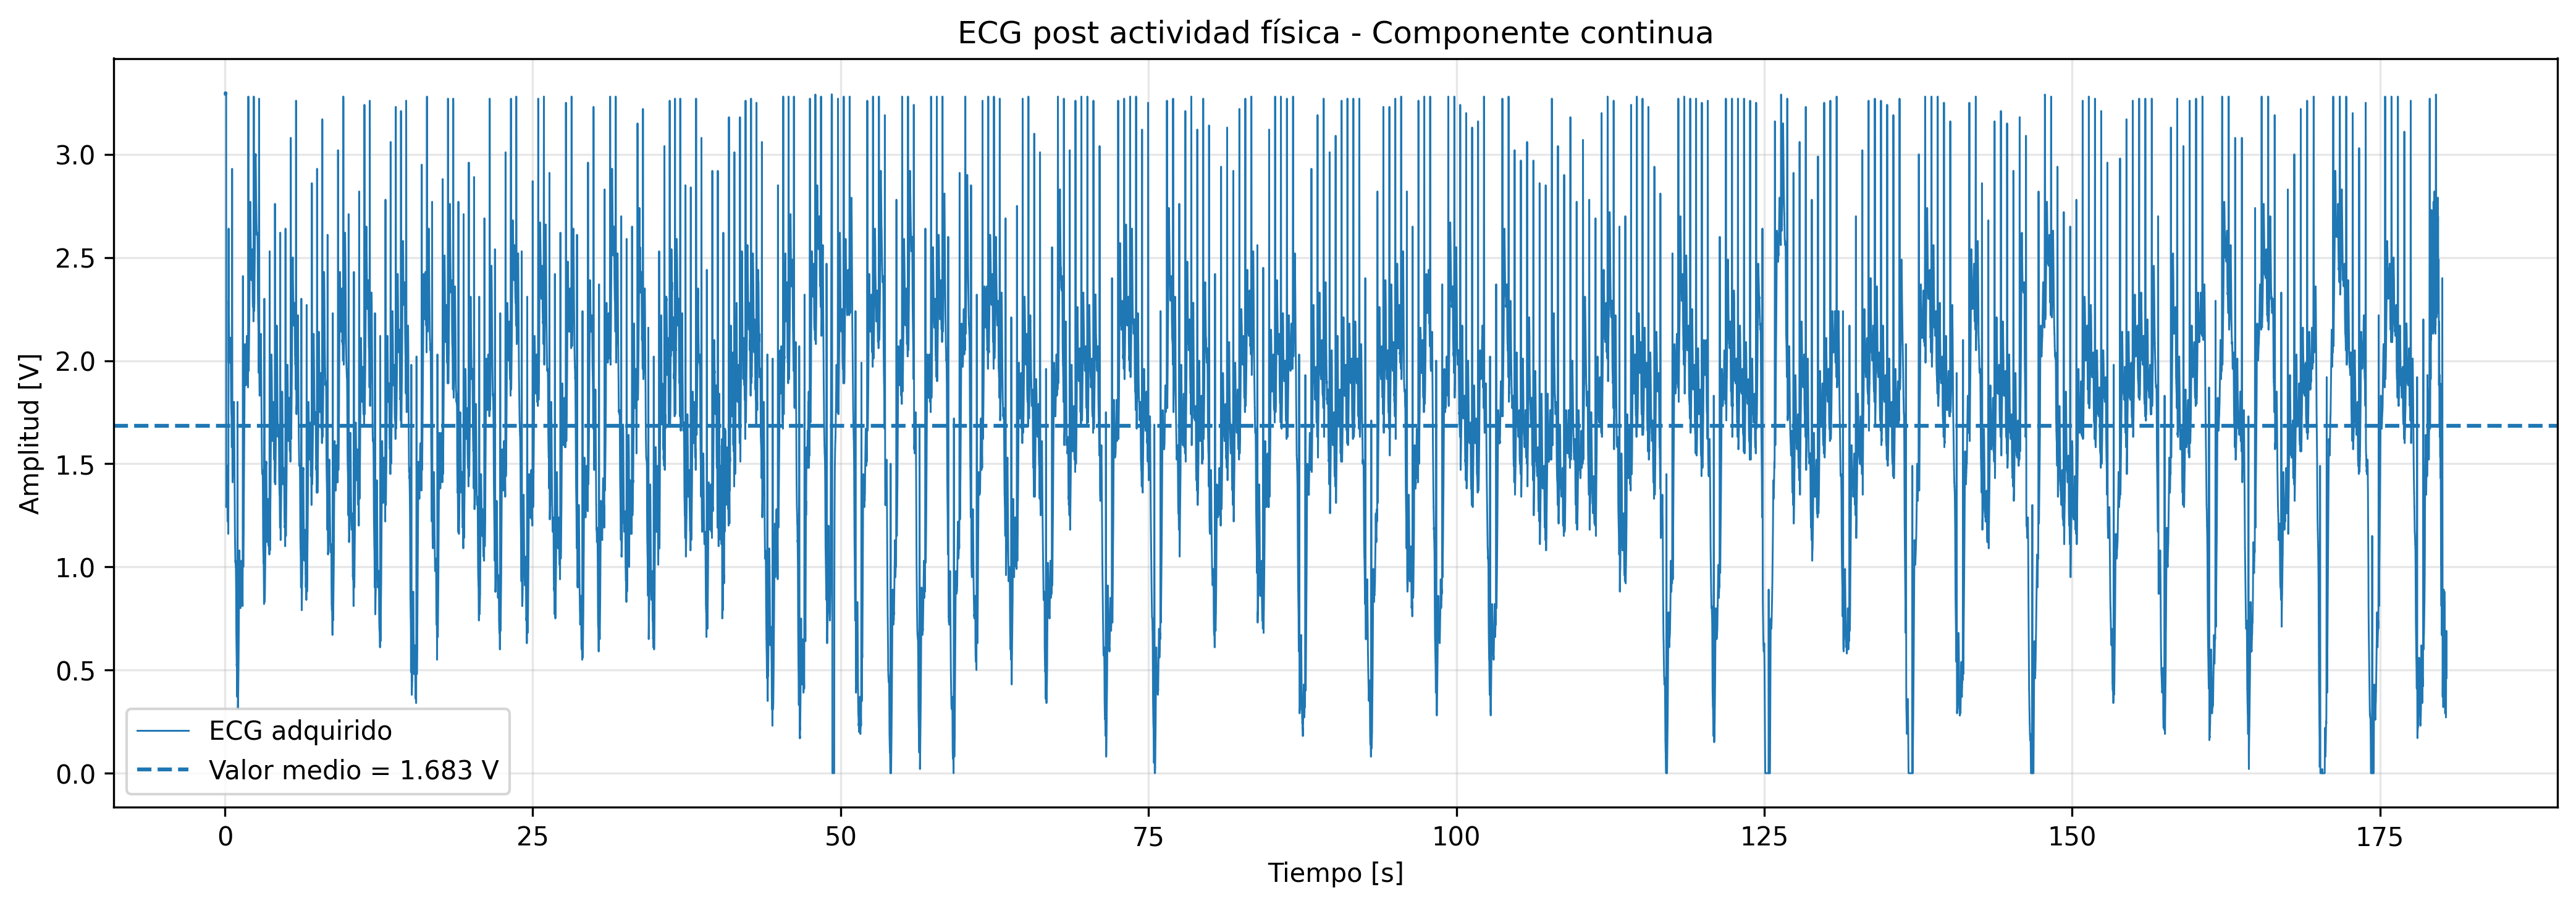
\includegraphics[width=0.95\textwidth]{Imagenes/ECG_Post_Offset.png}
    \caption{Señal de ECG posterior a la actividad física y valor medio del registro}
    \label{fig:offset-post}
\end{figure}

\FloatBarrier

Este desplazamiento permite confirmar la existencia de una componente de
continua asociada al sistema de adquisición. Sin embargo, en lugar de realizar
una resta independiente del valor medio y posteriormente aplicar otro método
para corregir la deriva, ambas componentes de muy baja frecuencia se eliminan
mediante una única etapa de filtrado pasa-altos.

La resta del valor medio se utiliza únicamente como referencia para visualizar
la señal centrada y facilitar la comparación con el resultado del filtrado.


\subsection{Corrección de la deriva mediante filtrado pasa-altos}

Para eliminar la componente continua y reducir las variaciones lentas de la
línea de base se utilizó un filtro IIR Butterworth pasa-altos de cuarto orden,
con una frecuencia de corte de

\[
f_c = 0.5~\mathrm{Hz}
\]

El filtro se aplicó en ambas direcciones temporales mediante un esquema
\textit{forward-backward}. De esta manera se obtiene una respuesta de fase
efectivamente nula, evitando introducir un desplazamiento temporal de los
complejos QRS.

Este aspecto es particularmente importante debido a que en los incisos
posteriores se utilizará la posición temporal de los picos R para calcular los
intervalos entre latidos.

Las Figuras~\ref{fig:hp-pre} y~\ref{fig:hp-post} muestran la comparación entre
las señales originales centradas únicamente para su visualización y las señales
obtenidas luego del filtro pasa-altos.

\begin{figure}[htbp]
    \centering
    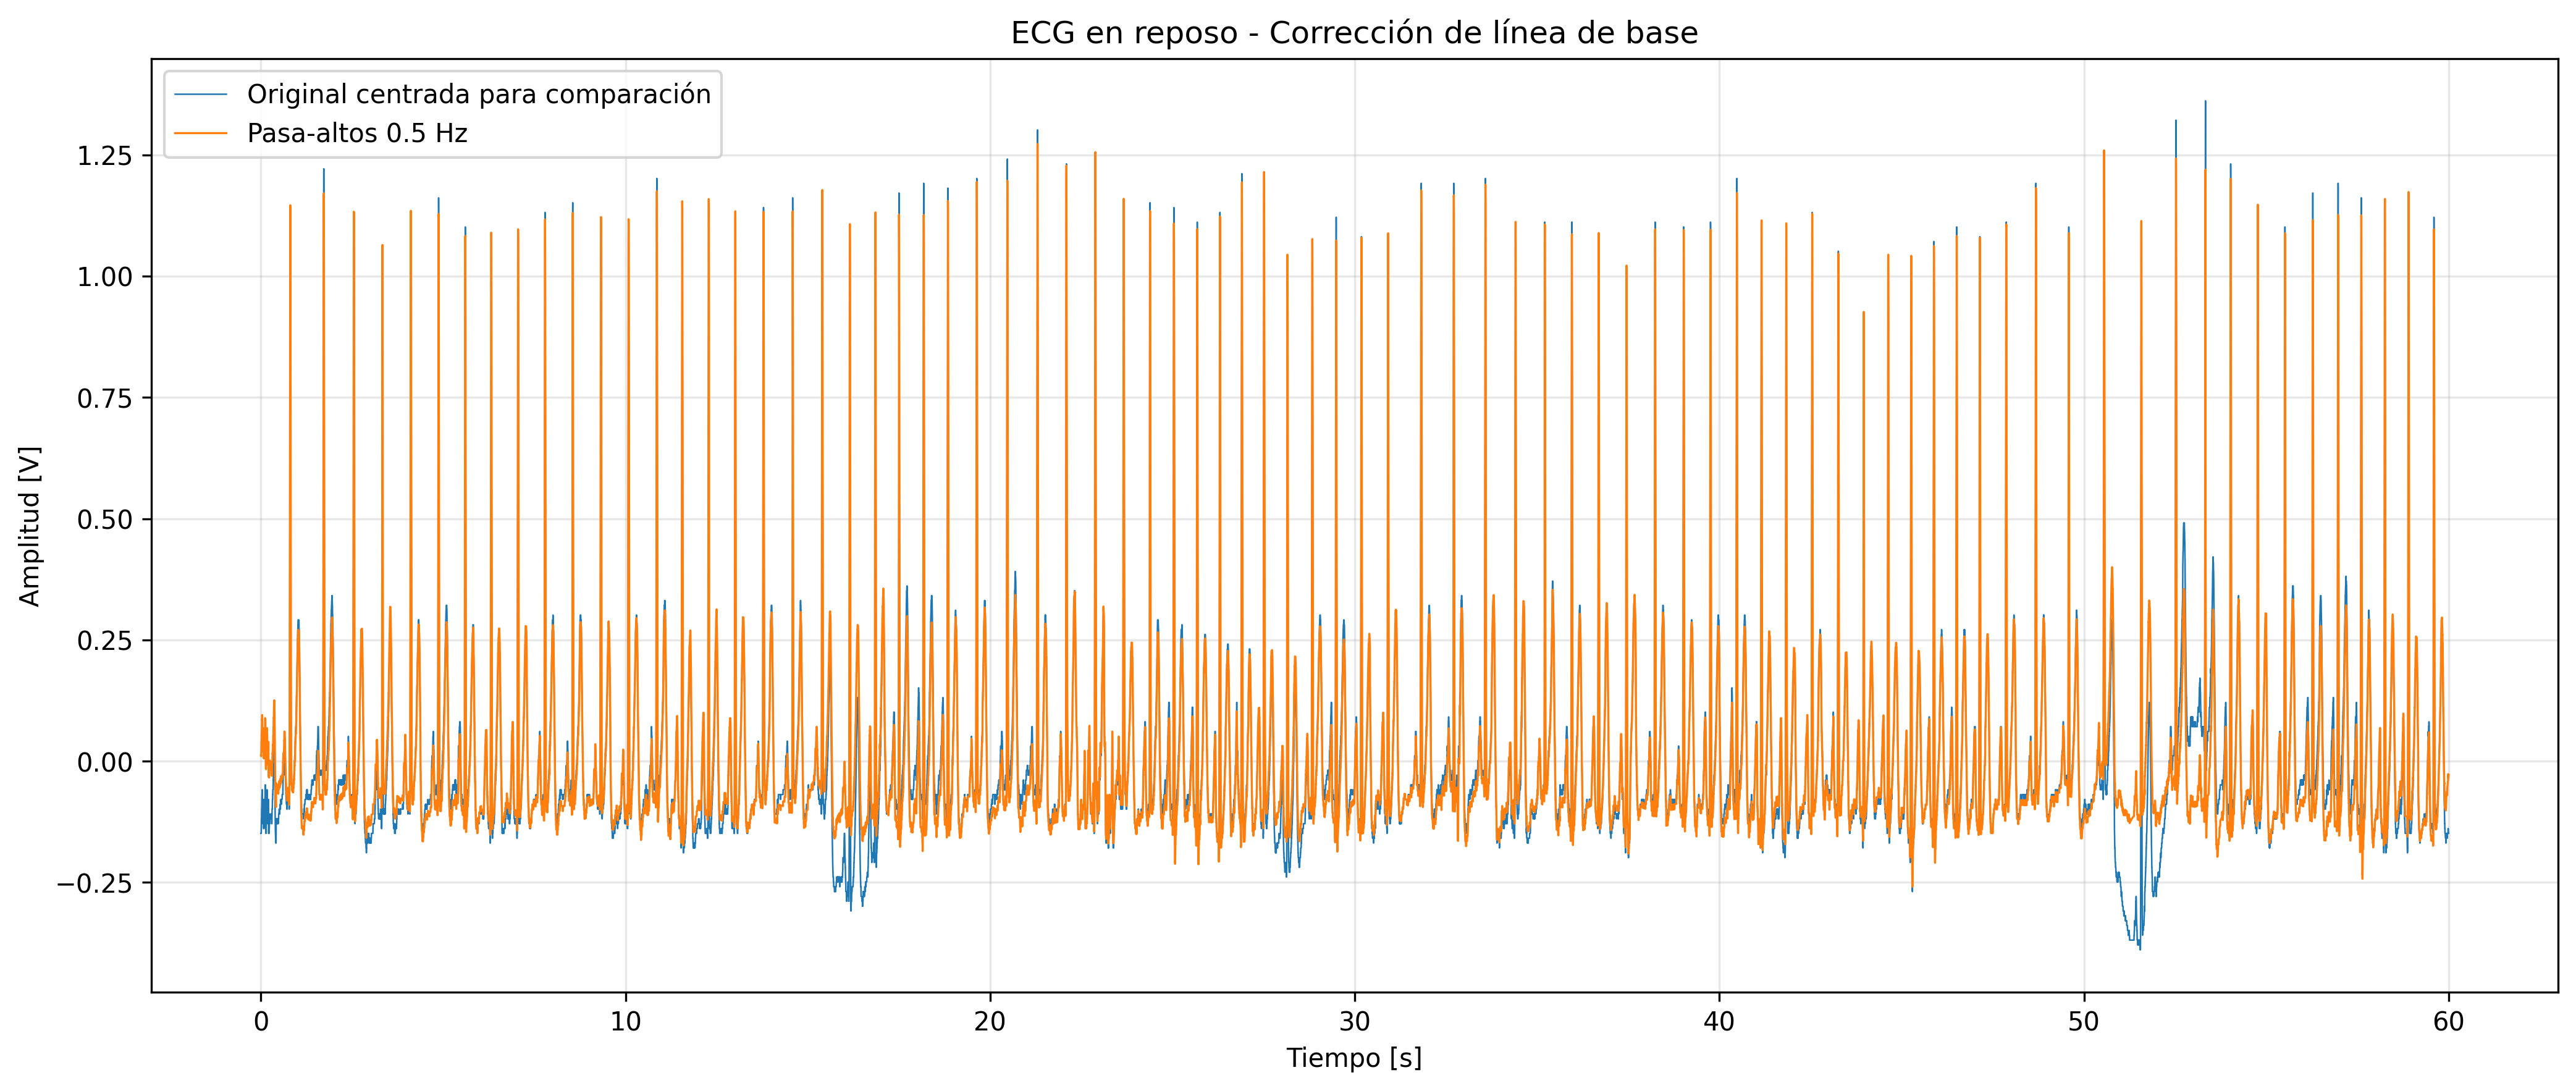
\includegraphics[width=0.95\textwidth]{Imagenes/ECG_Pre_PasaAltos.png}
    \caption{Efecto del filtro pasa-altos sobre el registro de ECG en reposo}
    \label{fig:hp-pre}
\end{figure}

\begin{figure}[htbp]
    \centering
    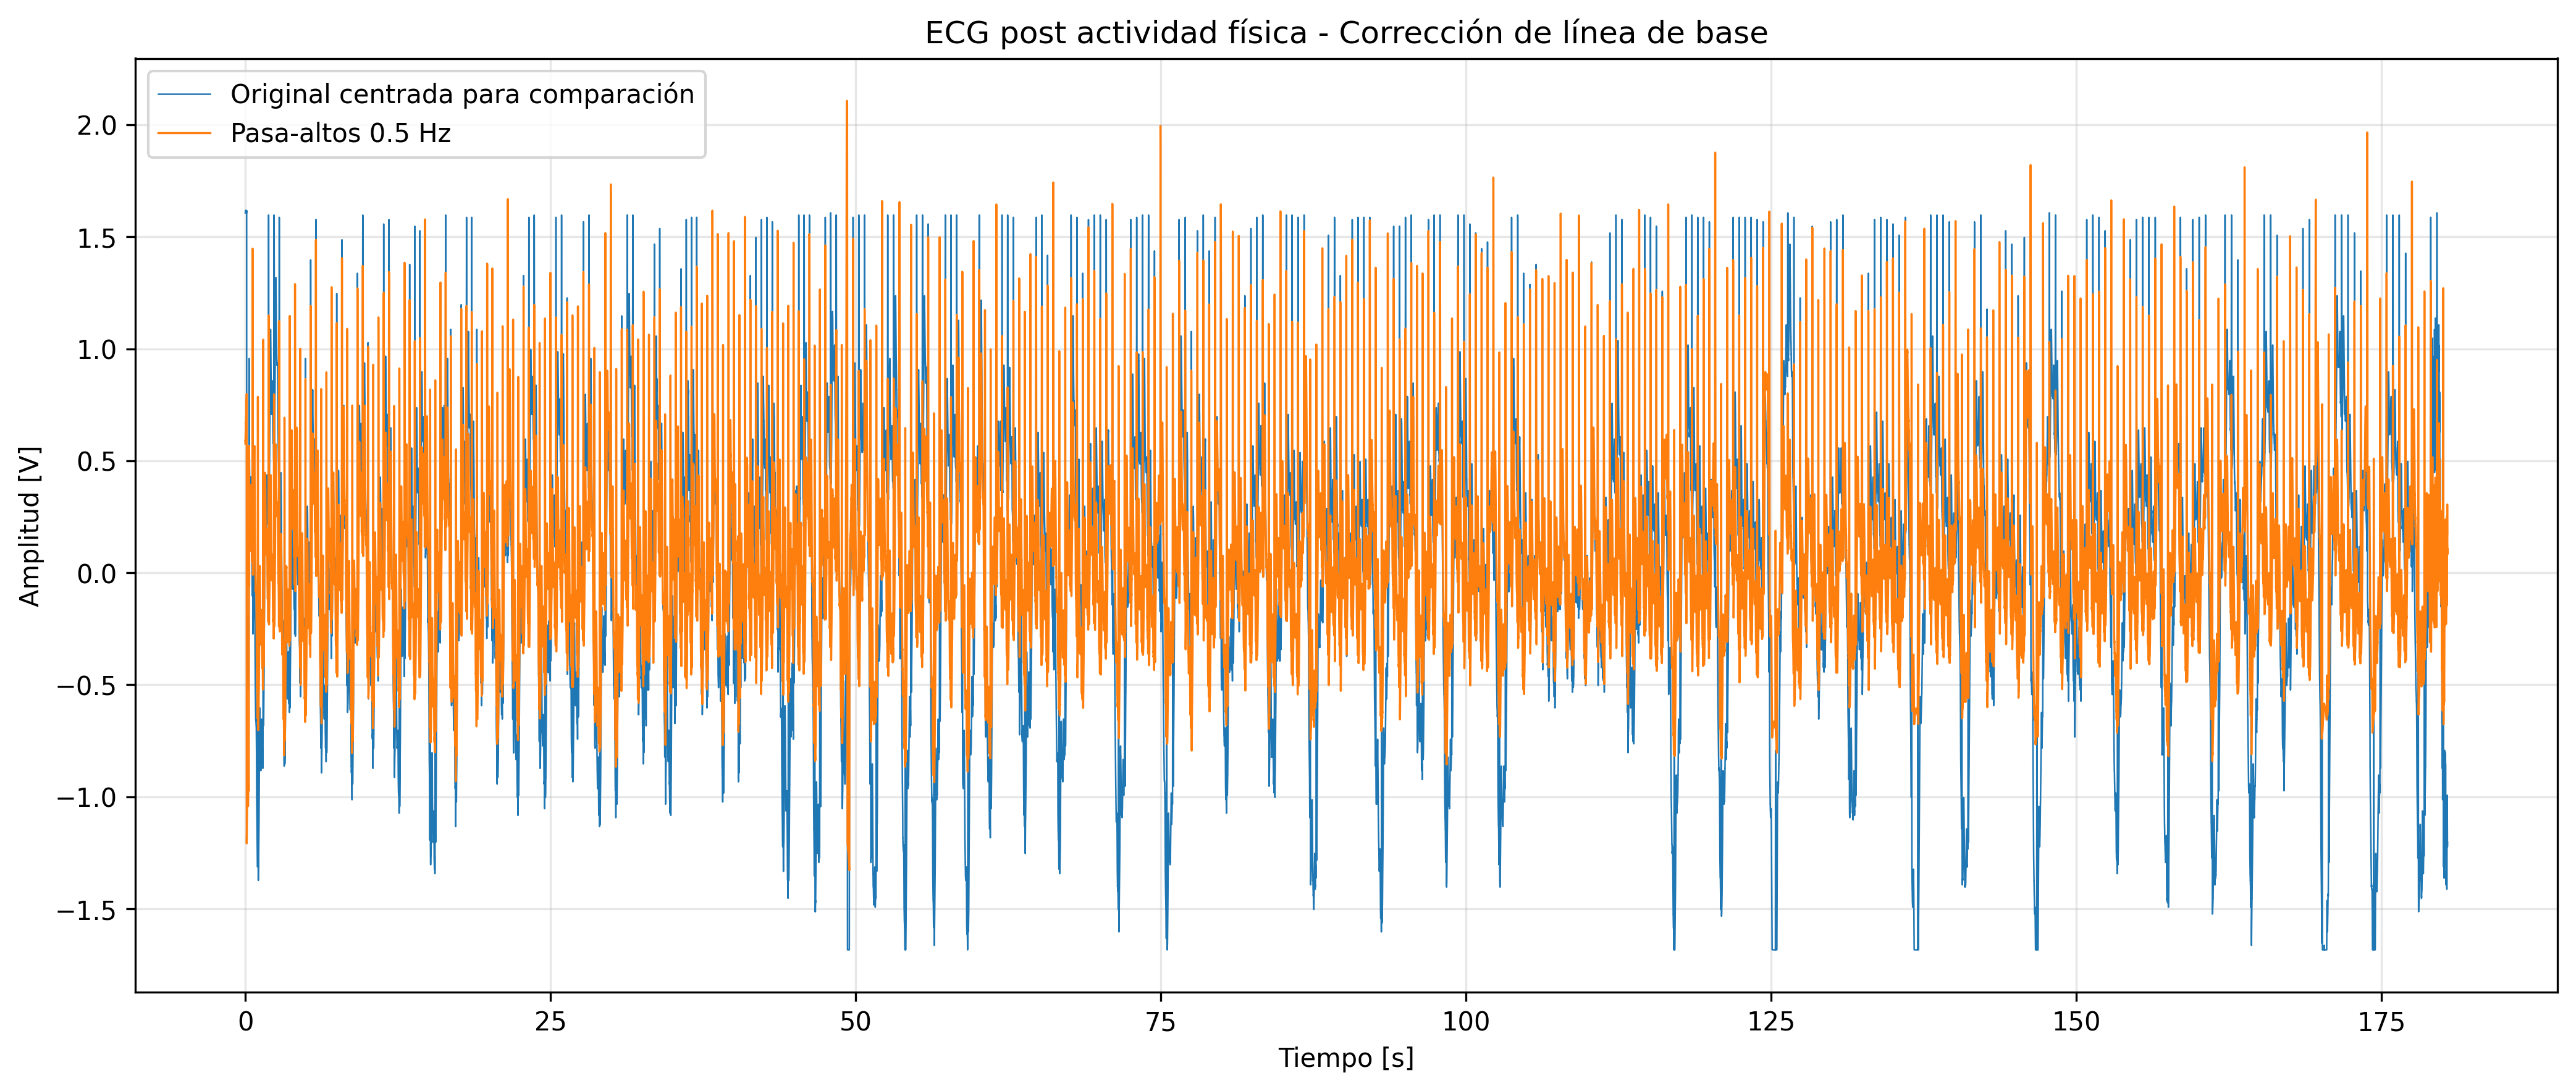
\includegraphics[width=0.95\textwidth]{Imagenes/ECG_Post_PasaAltos.png}
    \caption{Efecto del filtro pasa-altos sobre el registro posterior a la actividad física}
    \label{fig:hp-post}
\end{figure}

Para observar con mayor detalle el efecto del filtrado sobre la morfología de
los latidos se analizaron también ventanas temporales de diez segundos.

\begin{figure}[htbp]
    \centering
    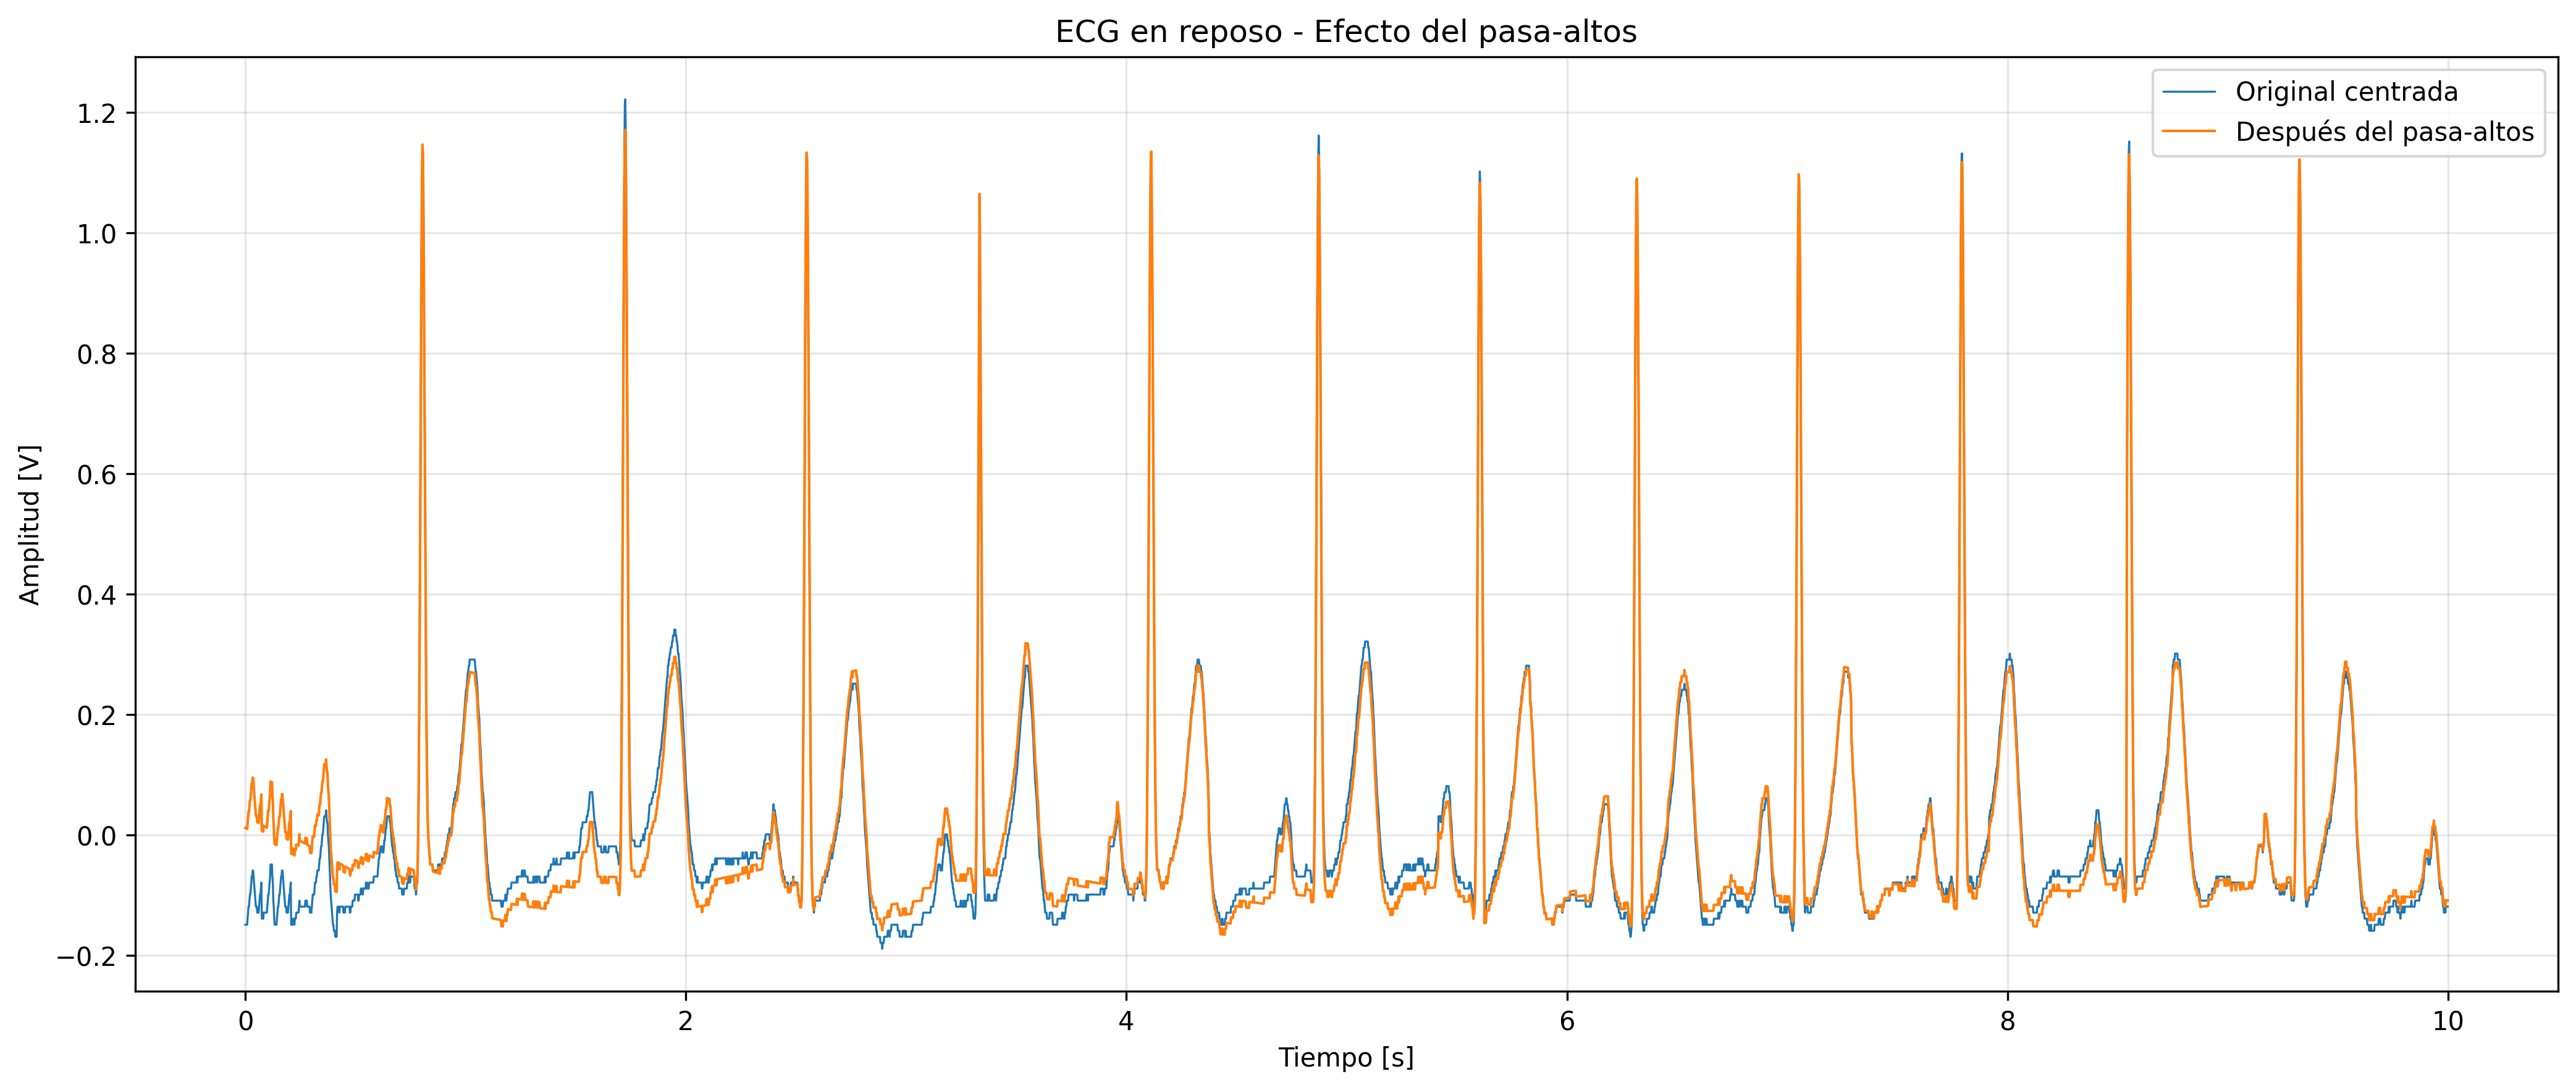
\includegraphics[width=0.95\textwidth]{Imagenes/ECG_Pre_PasaAltos_Zoom.png}
    \caption{Comparación ampliada antes y después del filtrado pasa-altos en el registro en reposo}
    \label{fig:hp-pre-zoom}
\end{figure}

\begin{figure}[htbp]
    \centering
    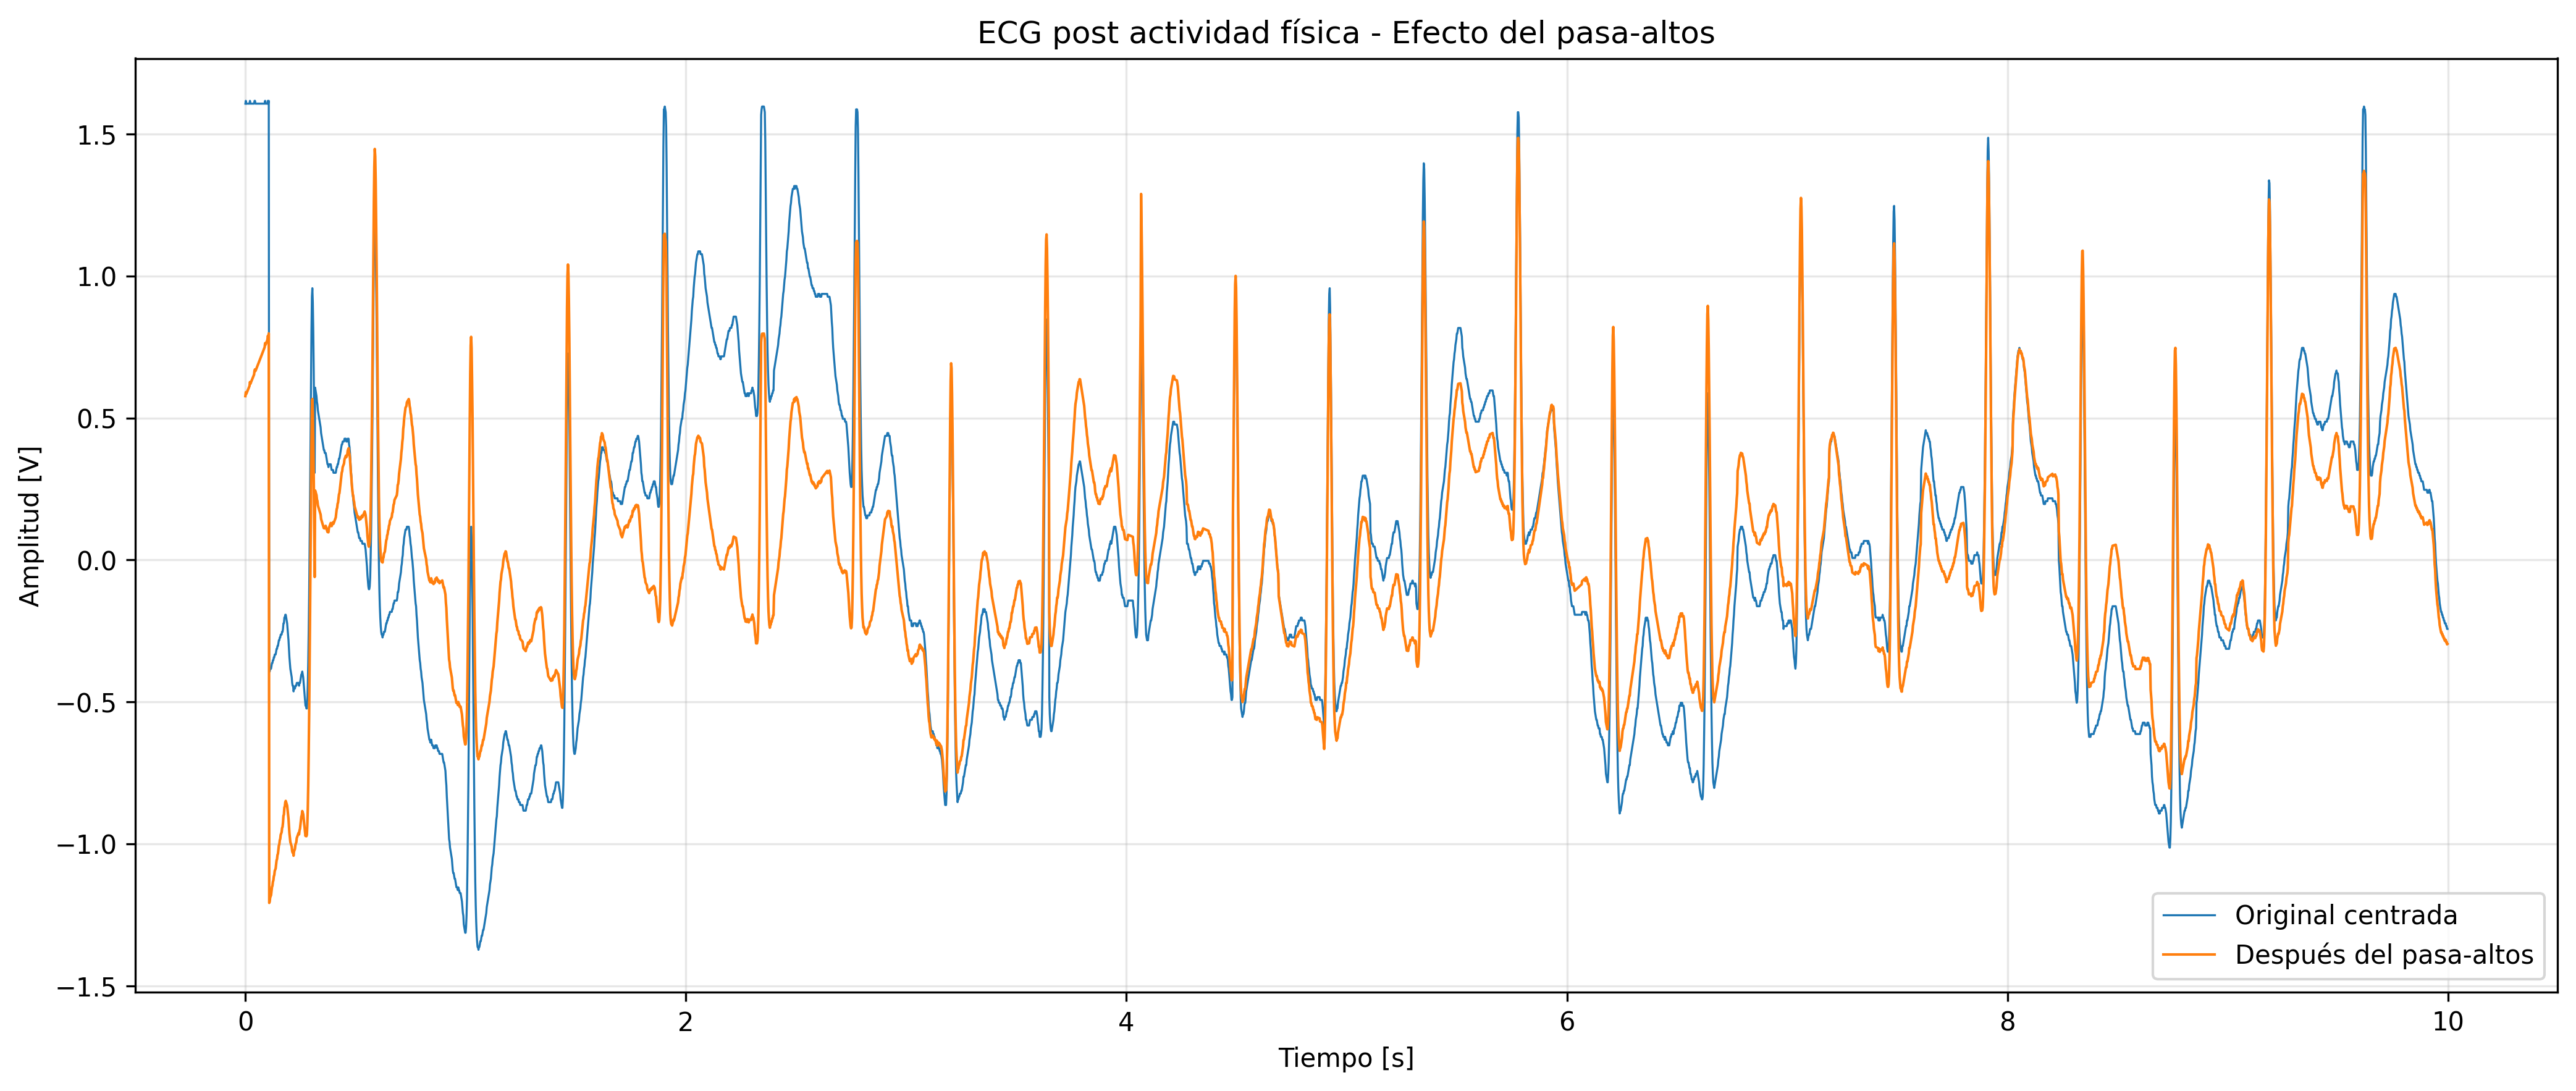
\includegraphics[width=0.95\textwidth]{Imagenes/ECG_Post_PasaAltos_Zoom.png}
    \caption{Comparación ampliada antes y después del filtrado pasa-altos en el registro posterior a la actividad física}
    \label{fig:hp-post-zoom}
\end{figure}

\FloatBarrier

Estas representaciones permiten evaluar simultáneamente la reducción de las
variaciones lentas de la línea de base y la conservación de las variaciones
rápidas asociadas a los complejos QRS.


\subsection{Análisis del contenido frecuencial}

Luego de corregir la línea de base se analizó el contenido frecuencial de las
señales mediante una estimación de la densidad espectral de potencia utilizando
el método de Welch.

El análisis se realizó luego del filtrado pasa-altos, de manera que la elevada
contribución de las componentes cercanas a continua no domine la
representación espectral.

En las Figuras~\ref{fig:psd-pre} y~\ref{fig:psd-post} se muestran las densidades
espectrales de potencia obtenidas para ambos registros dentro del intervalo de
0 a 100 Hz.

\begin{figure}[htbp]
    \centering
    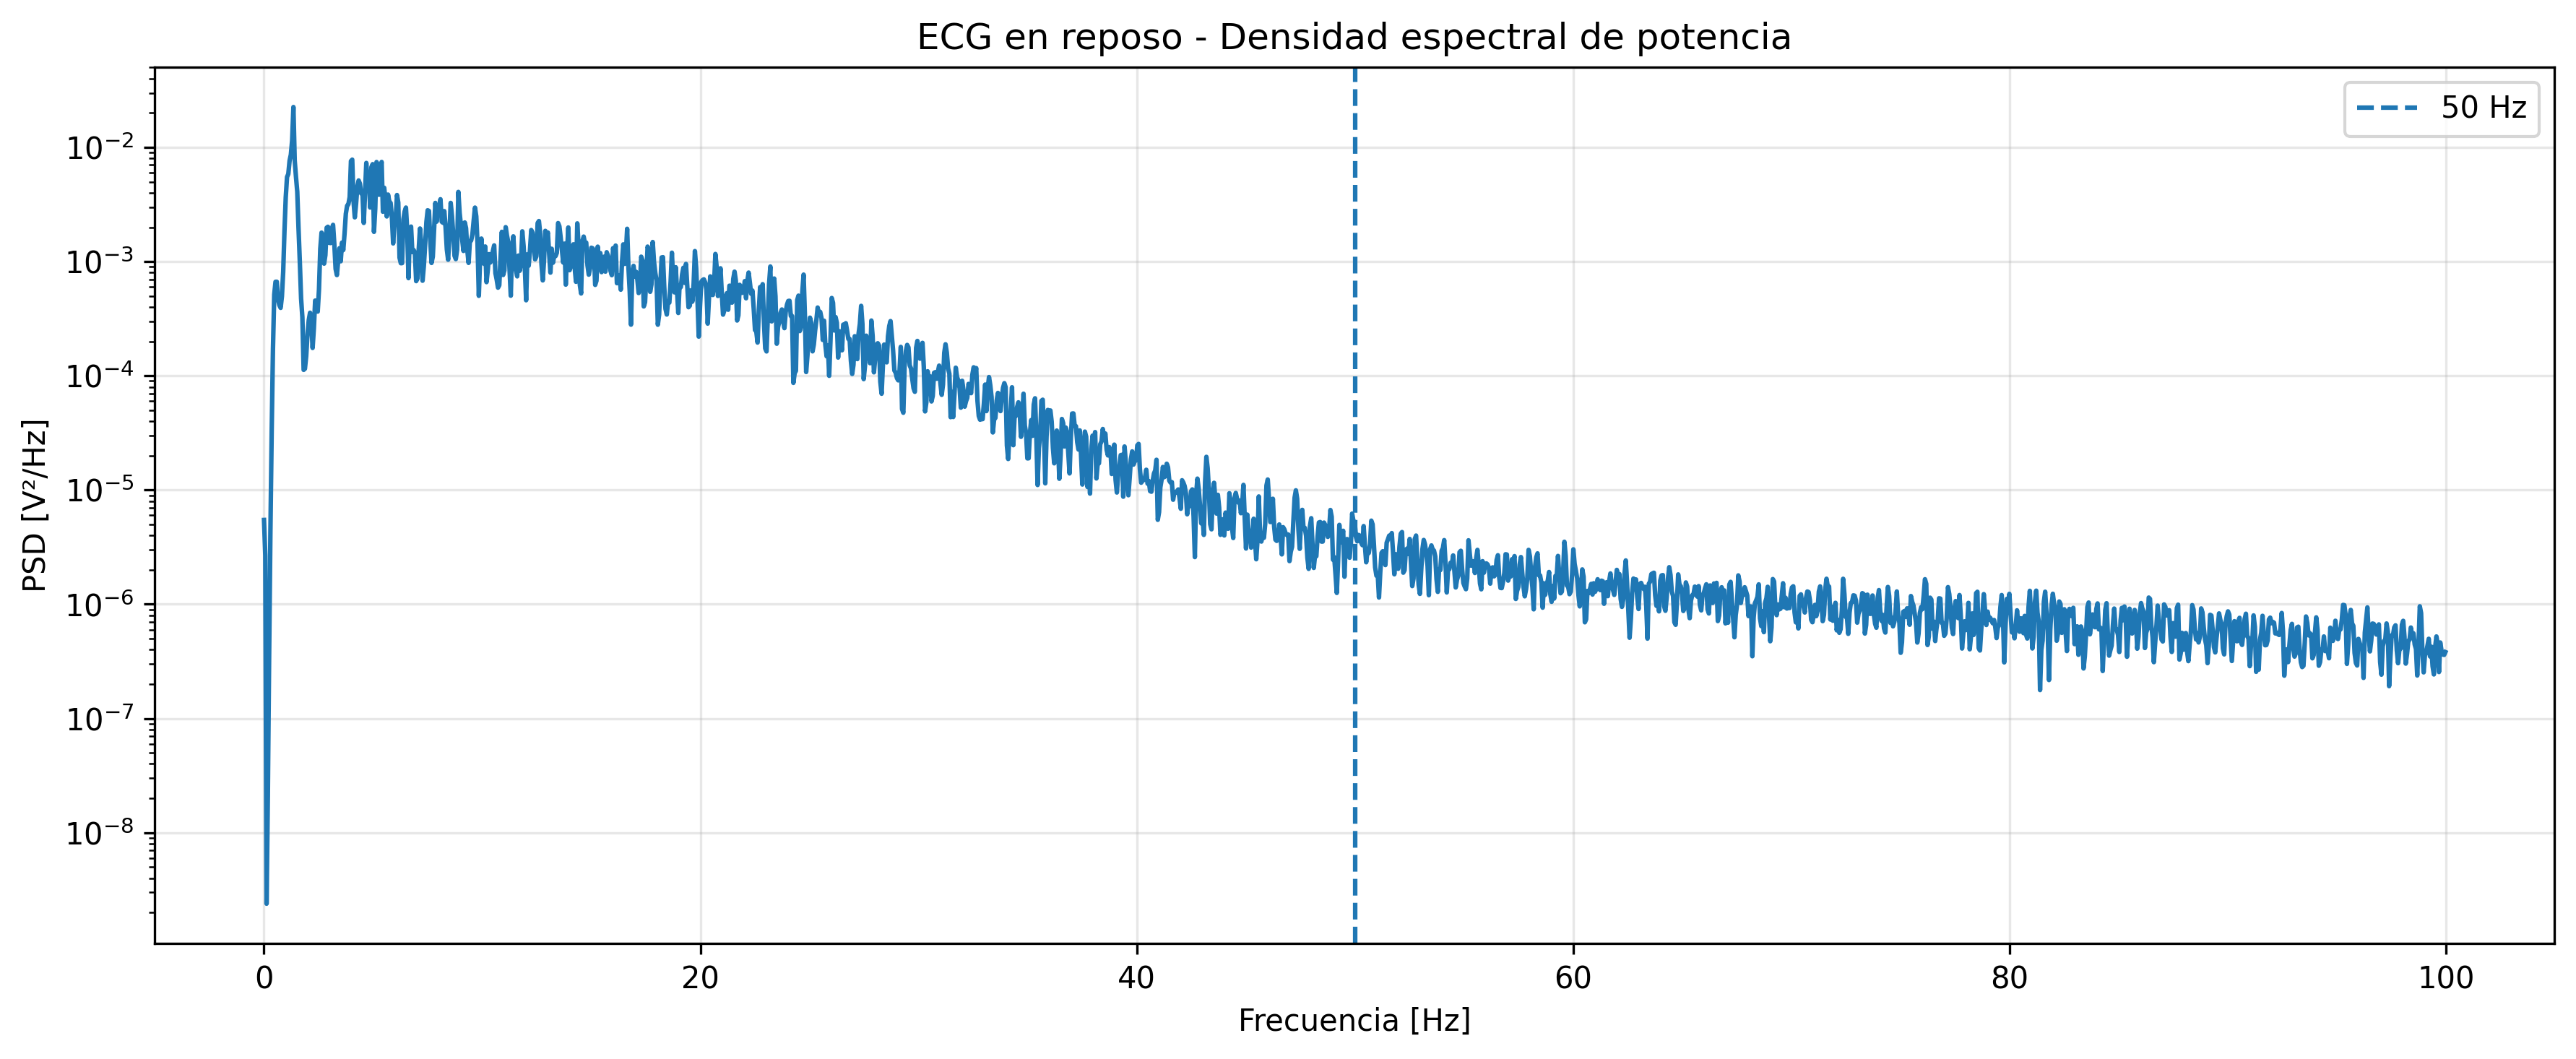
\includegraphics[width=0.90\textwidth]{Imagenes/ECG_Pre_PSD.png}
    \caption{Densidad espectral de potencia del ECG registrado en reposo}
    \label{fig:psd-pre}
\end{figure}

\begin{figure}[htbp]
    \centering
    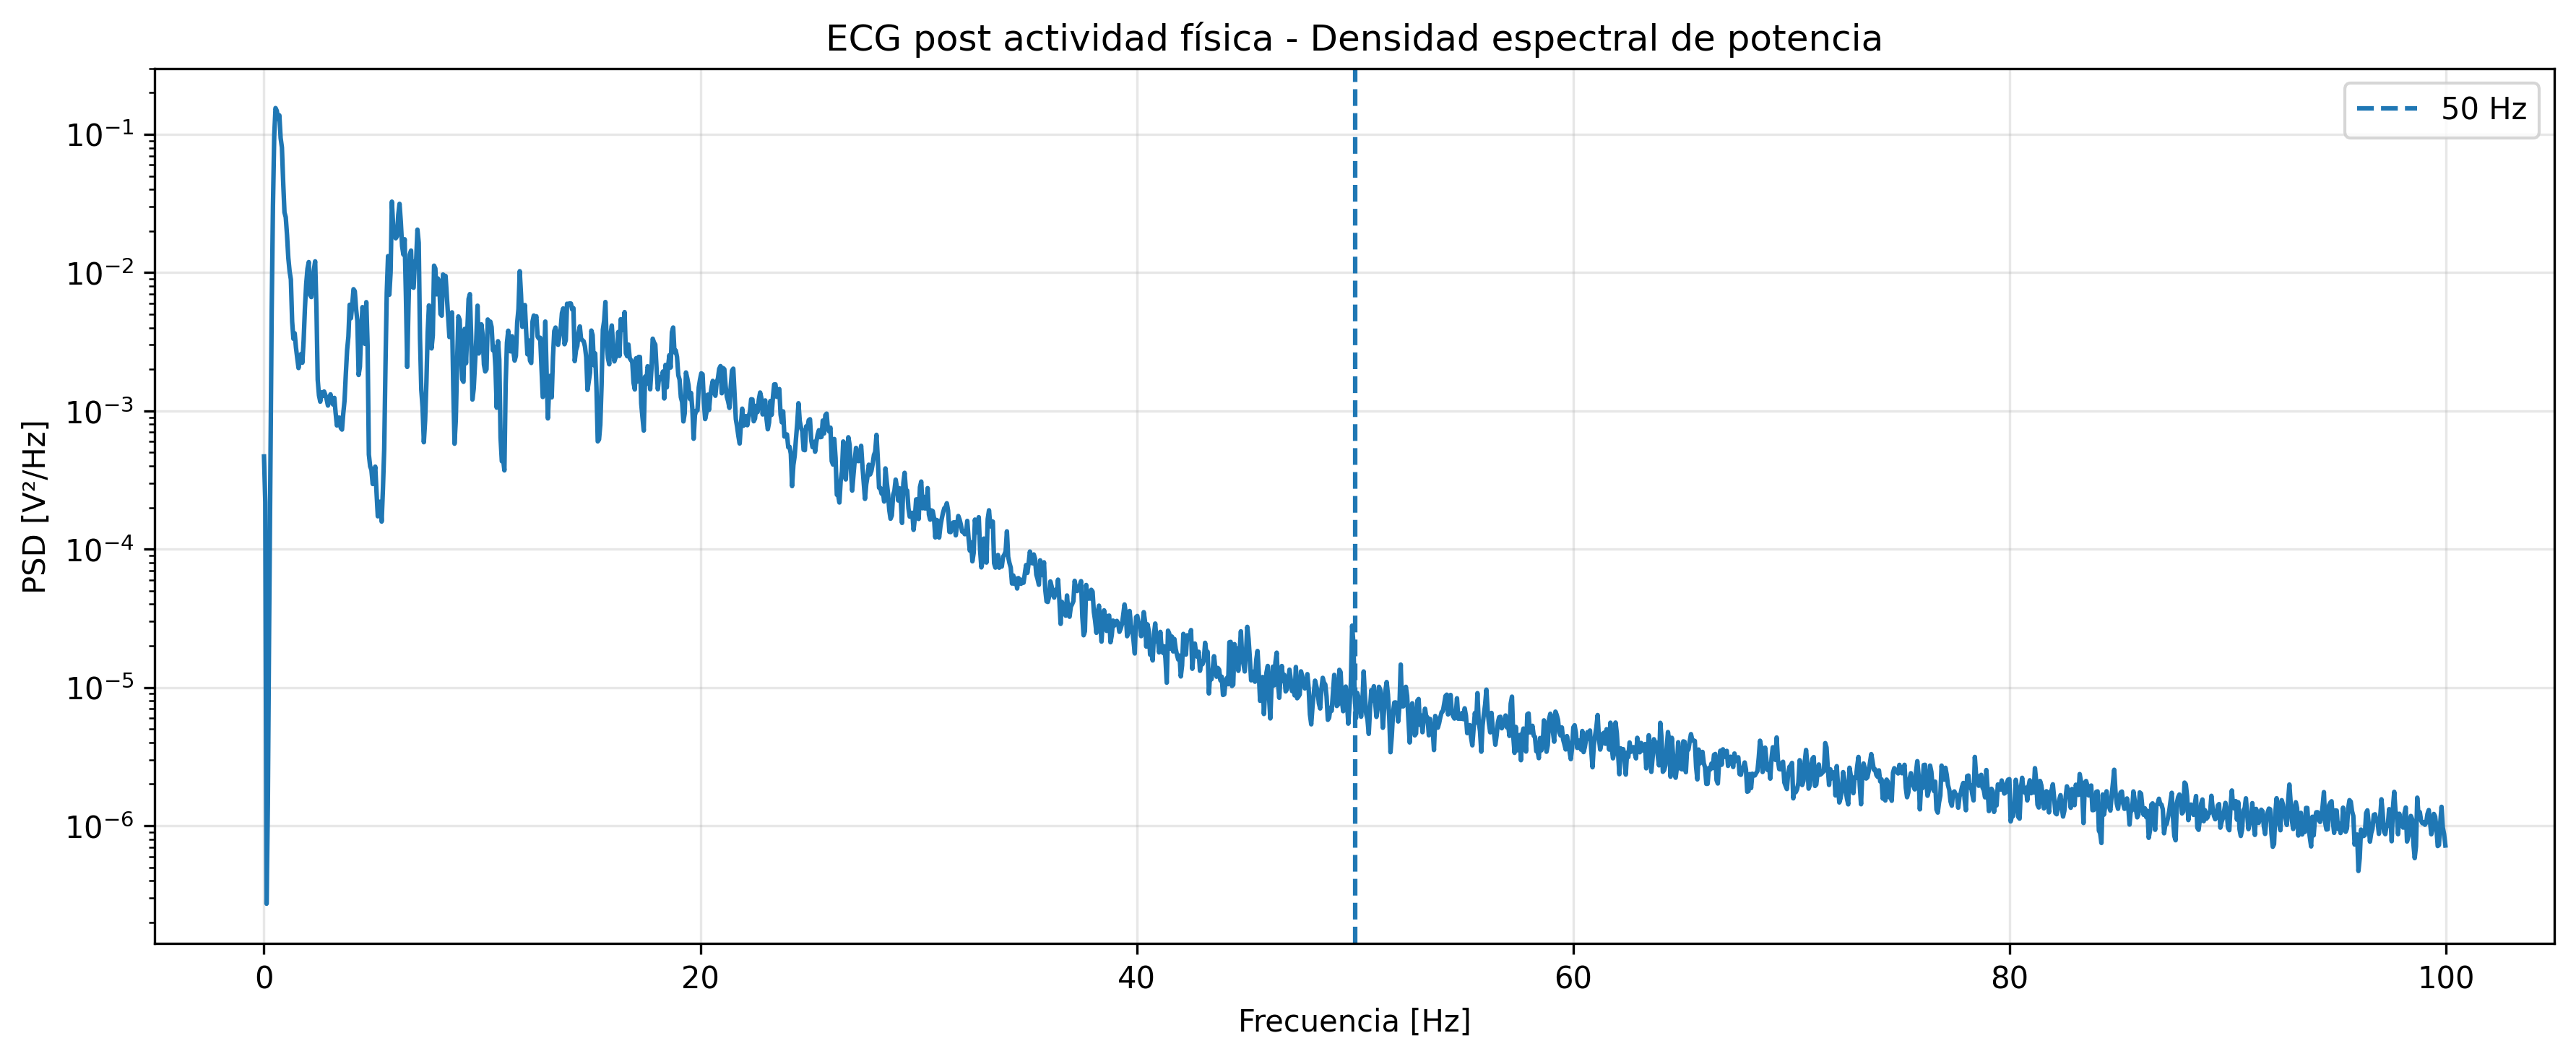
\includegraphics[width=0.90\textwidth]{Imagenes/ECG_Post_PSD.png}
    \caption{Densidad espectral de potencia del ECG registrado luego de la actividad física}
    \label{fig:psd-post}
\end{figure}

\FloatBarrier

El objetivo de esta representación fue identificar la distribución frecuencial
de la señal y evaluar particularmente la posible existencia de componentes
estrechas asociadas a interferencia eléctrica.

A partir de las densidades espectrales obtenidas no se observa una componente
de potencia considerable concentrada en 50 Hz. Por este motivo, se decidió no
aplicar un filtro \textit{notch}, ya que su utilización no aportaría una mejora
significativa a la señal y podría modificar innecesariamente componentes
frecuenciales cercanas.

De manera análoga, tampoco se aplicó en esta etapa un filtro pasa-bajos
adicional. Las representaciones espectrales no muestran que el ruido de alta
frecuencia constituya una perturbación predominante en los registros, por lo
que se consideró innecesario incorporar una nueva etapa de filtrado.

Además, en la etapa posterior de detección de complejos QRS mediante el
algoritmo de Pan--Tompkins se aplicará un filtro pasa-banda específico entre
5 Hz y 15 Hz. Dicho filtrado tiene como objetivo realzar el contenido
frecuencial asociado a los complejos QRS y atenuar otras componentes de la
señal. Por lo tanto, aplicar previamente un filtro pasa-bajos adicional
introduciría una etapa de procesamiento que no resulta necesaria para el
objetivo de este trabajo.

En consecuencia, luego del análisis espectral se mantuvo como única etapa de
filtrado de acondicionamiento el filtro pasa-altos de 0.5 Hz utilizado para
reducir la componente continua y la deriva de la línea de base.

\subsection{Identificación de saturaciones}

Además del filtrado, se identificaron las muestras que alcanzan valores
próximos a los límites del rango de adquisición.

Se consideraron como posibles muestras saturadas aquellas que cumplen

\[
x[n] \leq 0.01~\mathrm{V}
\]

o bien

\[
x[n] \geq 3.29~\mathrm{V}
\]

En las Figuras~\ref{fig:saturacion-pre} y~\ref{fig:saturacion-post} se muestran
las muestras que cumplen este criterio para cada uno de los registros.

\begin{figure}[htbp]
    \centering
    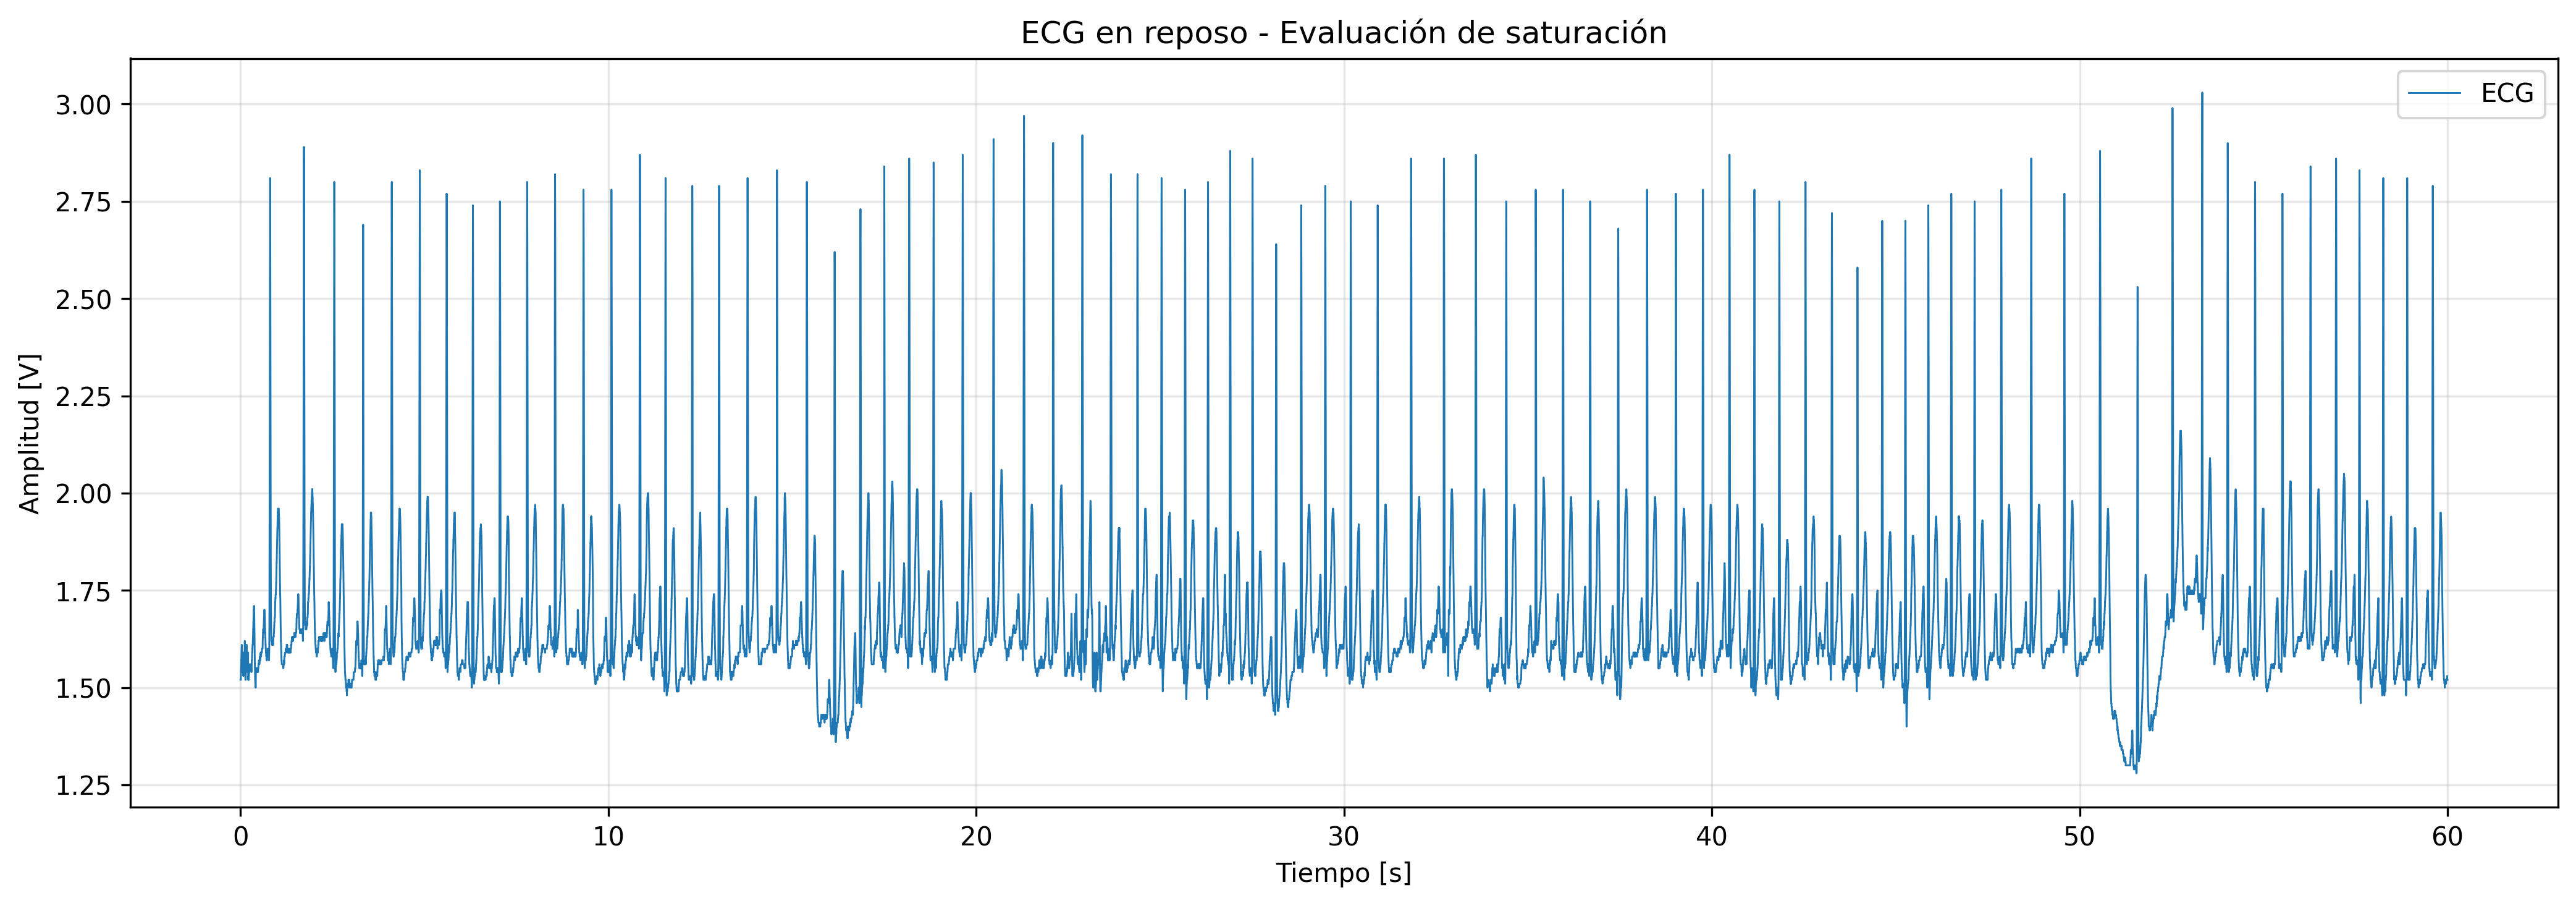
\includegraphics[width=0.95\textwidth]{Imagenes/ECG_Pre_Saturacion.png}
    \caption{Evaluación de posibles saturaciones en el registro de ECG en reposo}
    \label{fig:saturacion-pre}
\end{figure}

\begin{figure}[htbp]
    \centering
    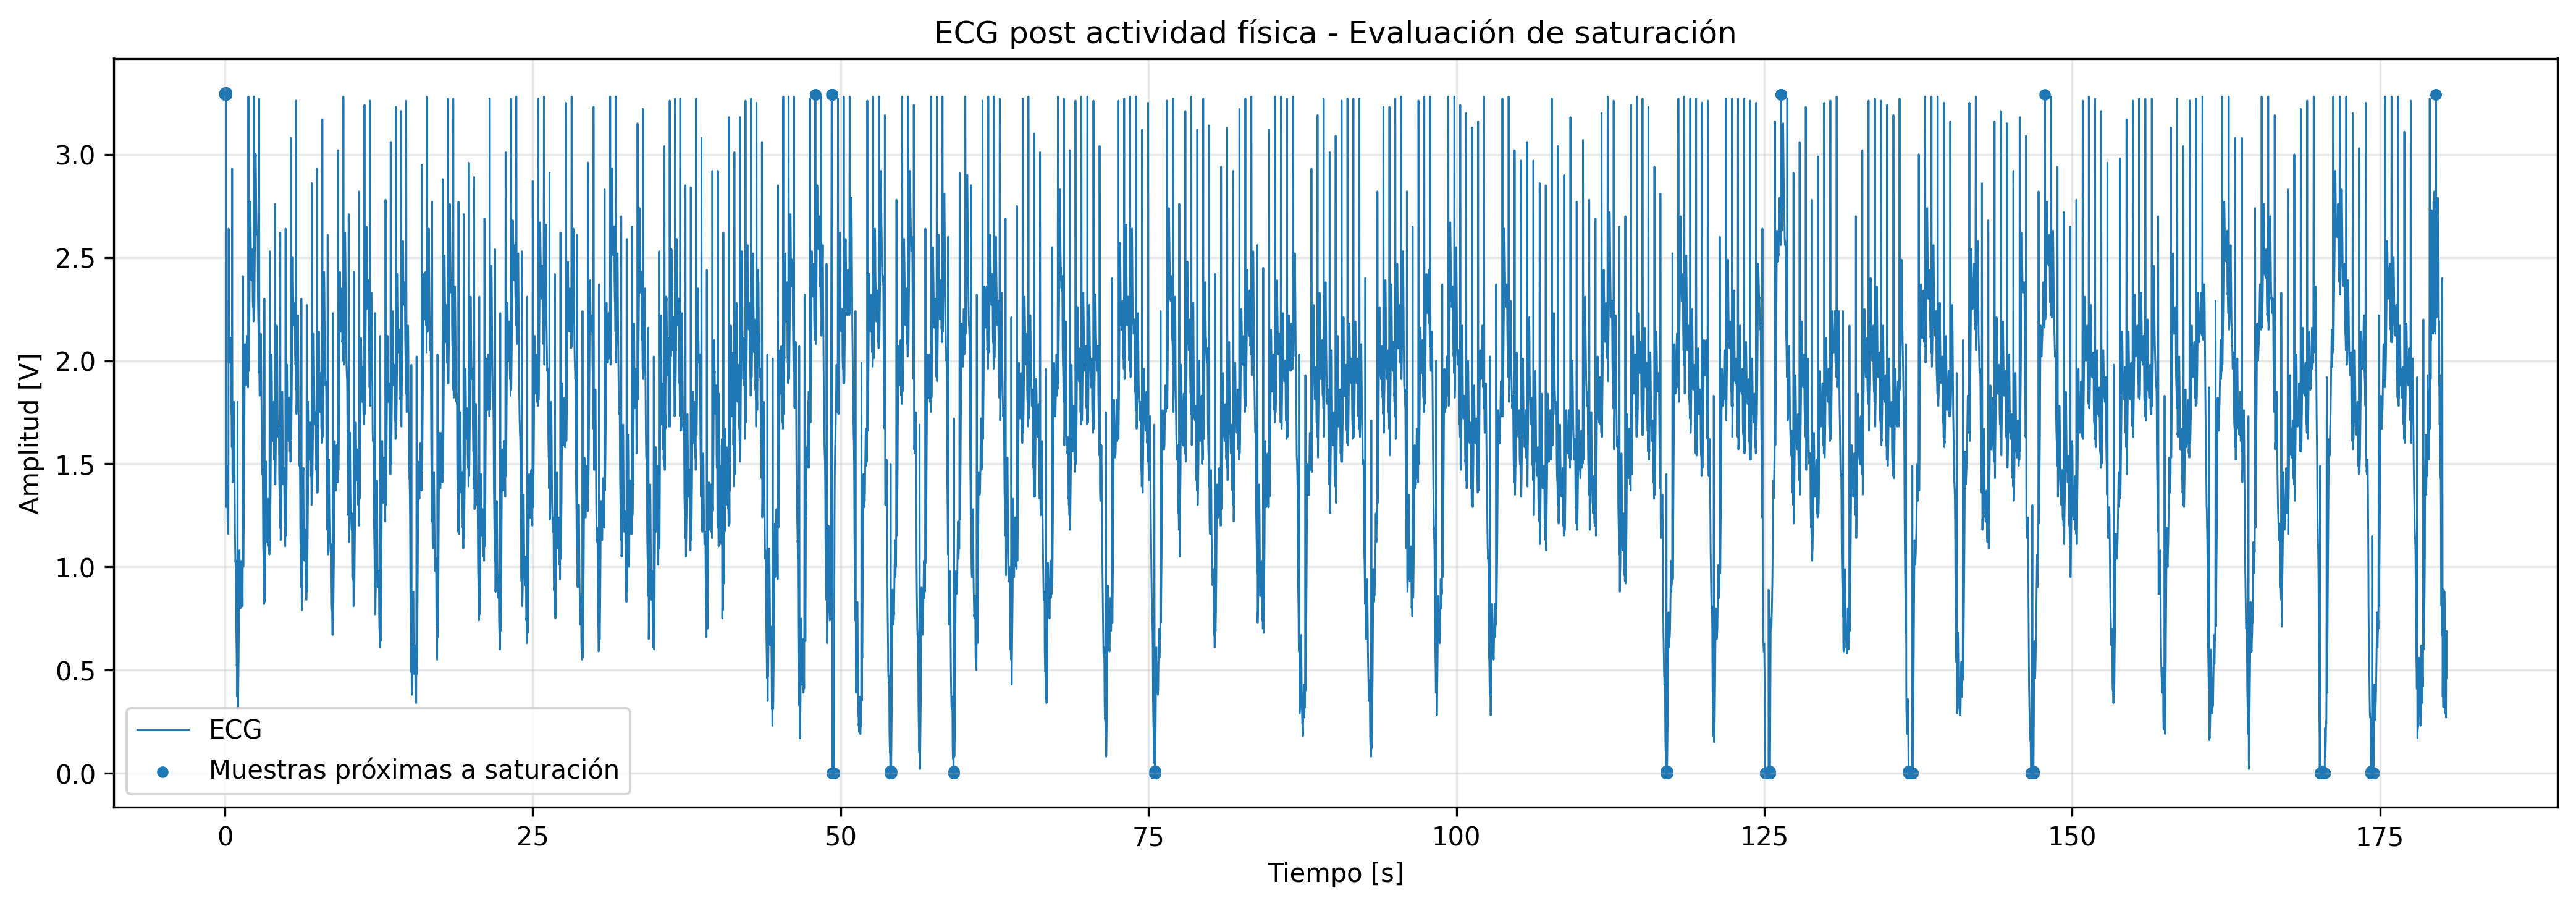
\includegraphics[width=0.95\textwidth]{Imagenes/ECG_Post_Saturacion.png}
    \caption{Evaluación de posibles saturaciones en el registro posterior a la actividad física}
    \label{fig:saturacion-post}
\end{figure}

\FloatBarrier

La identificación de estos segmentos no implica su corrección mediante
filtrado. Cuando el sistema de adquisición alcanza alguno de sus límites se
produce una pérdida de información que no puede recuperarse mediante
procesamiento digital.

Por este motivo, estas muestras se conservaron identificadas para poder
considerarlas posteriormente durante la detección de los complejos QRS.


\subsection{Resultado del preprocesamiento}

Luego de aplicar el filtro pasa-altos para corregir la componente continua y
la deriva de la línea de base, y de verificar mediante el análisis espectral
que no resultaba necesario incorporar un filtro \textit{notch} ni un filtro
pasa-bajos adicional, se obtuvieron las señales preprocesadas que serán
utilizadas en las etapas posteriores del trabajo.

Las señales resultantes se muestran en las
Figuras~\ref{fig:procesado-pre} y~\ref{fig:procesado-post}.

\begin{figure}[htbp]
    \centering
    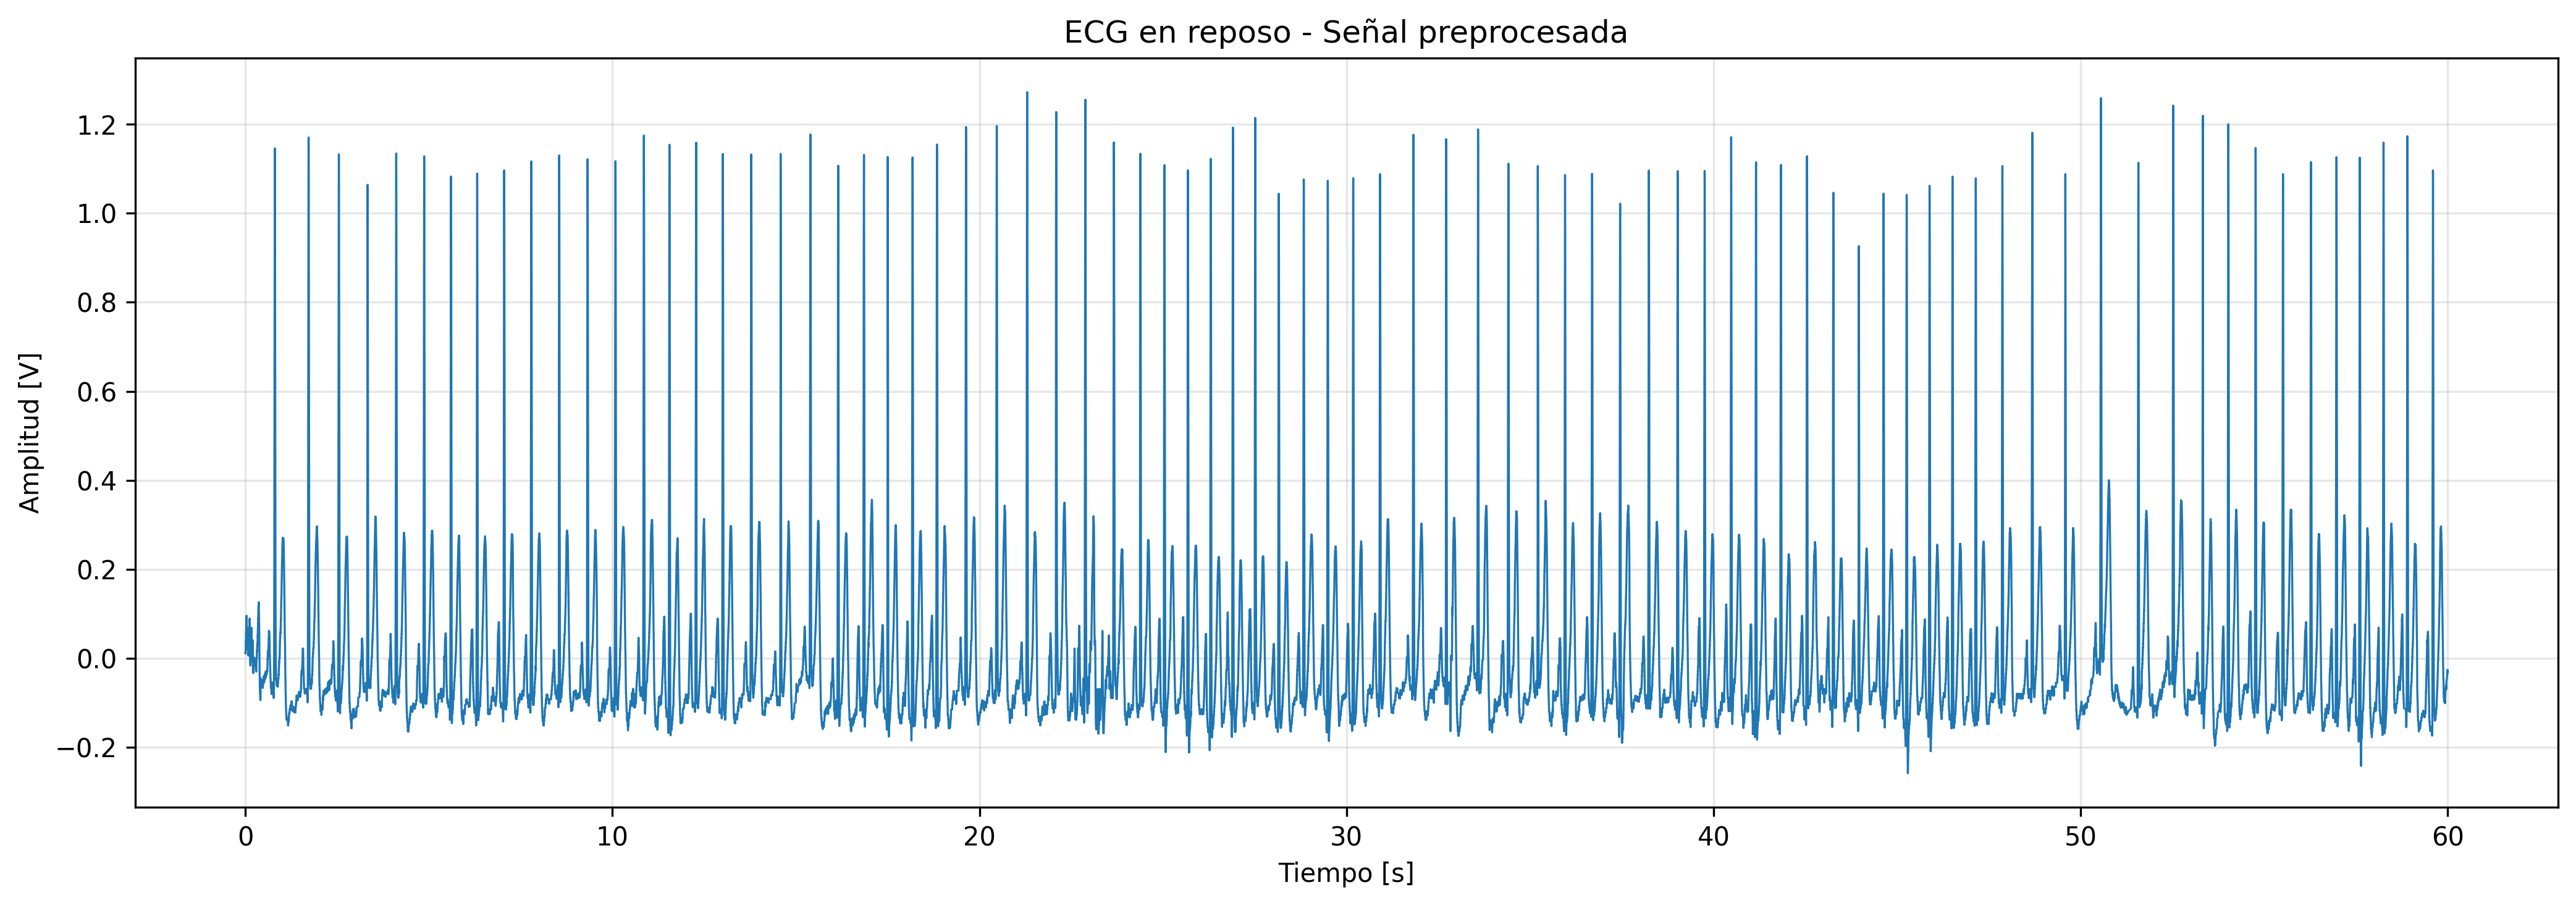
\includegraphics[width=0.95\textwidth]{Imagenes/ECG_Pre_Procesado.png}
    \caption{Señal de ECG en reposo luego del preprocesamiento}
    \label{fig:procesado-pre}
\end{figure}

\begin{figure}[htbp]
    \centering
    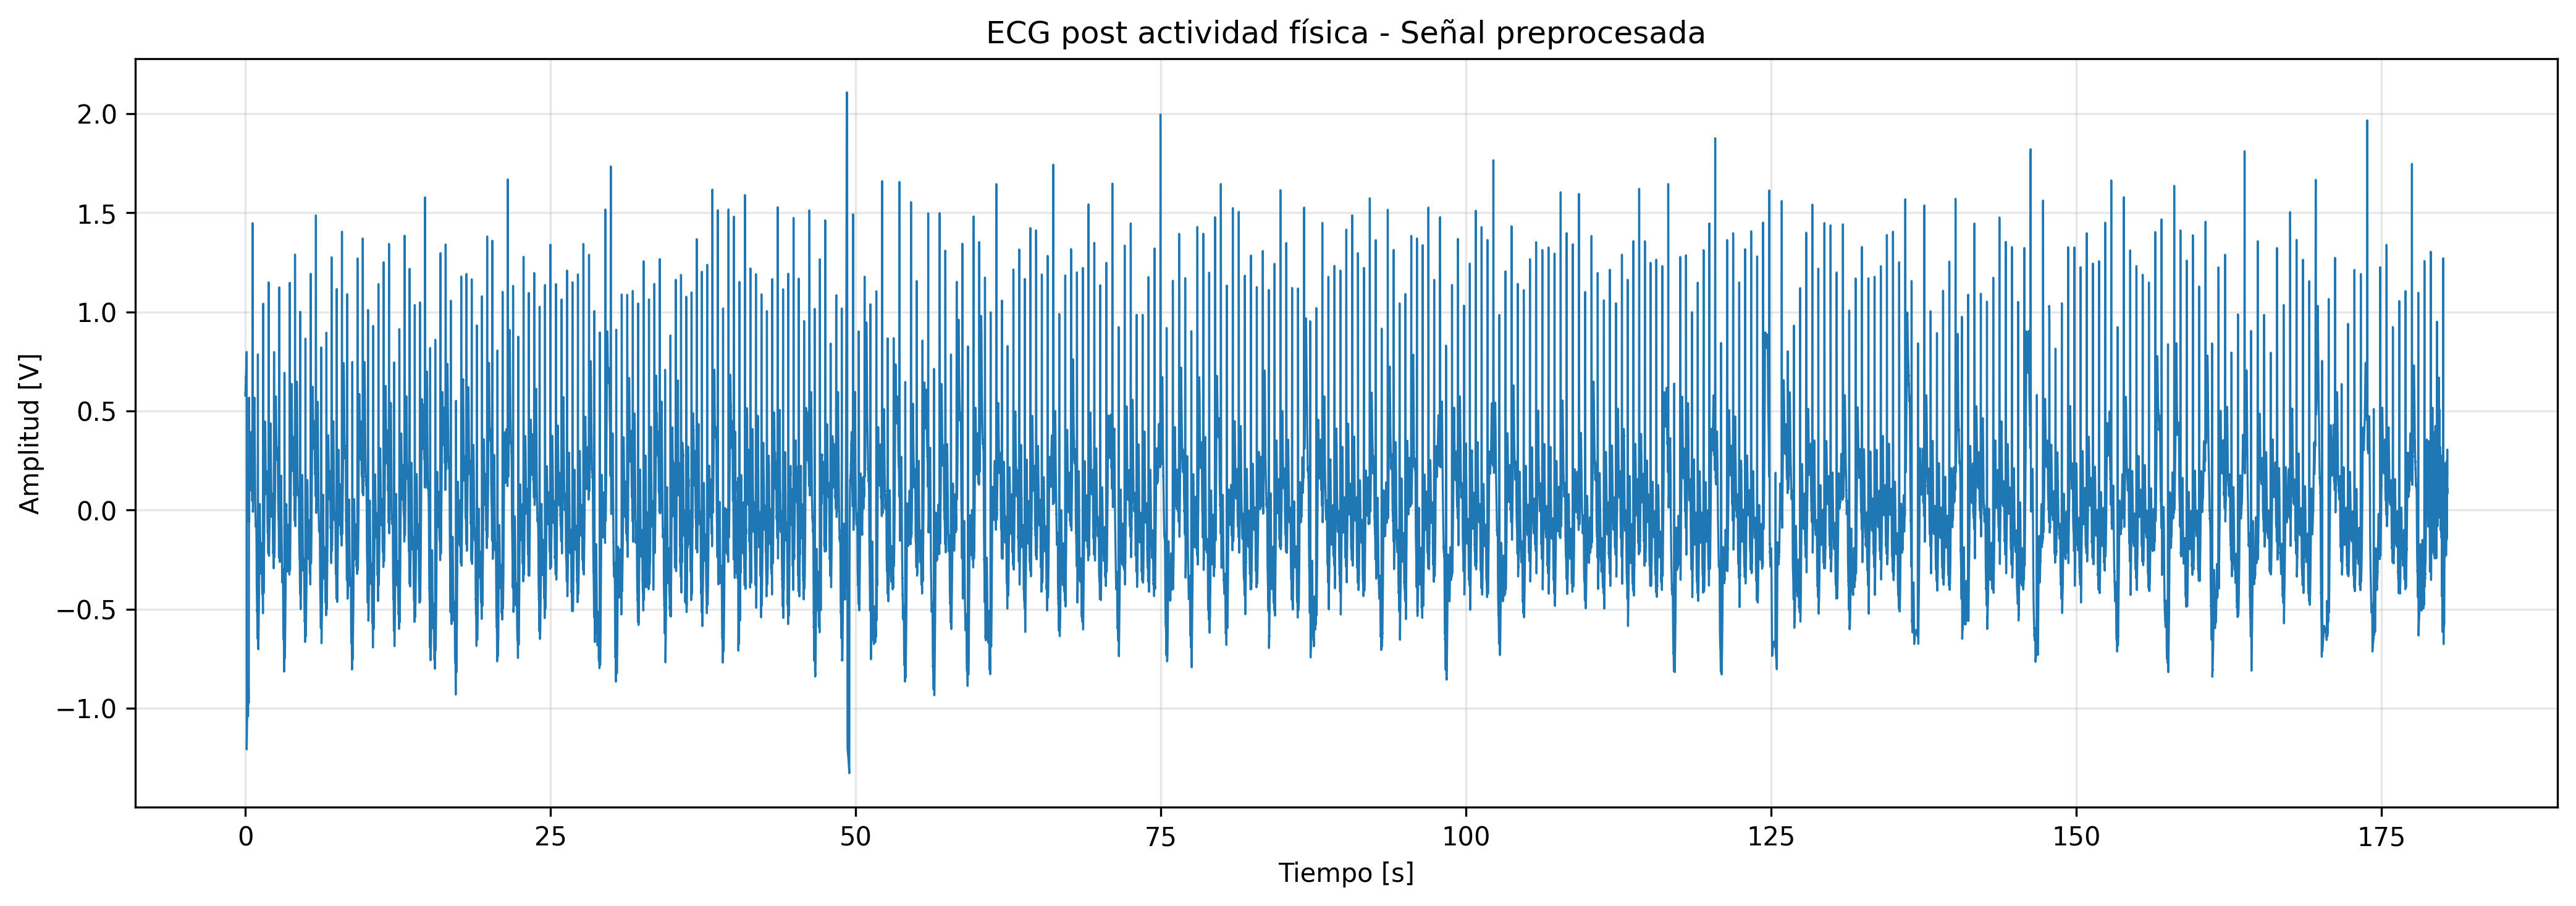
\includegraphics[width=0.95\textwidth]{Imagenes/ECG_Post_Procesado.png}
    \caption{Señal de ECG posterior a la actividad física luego del preprocesamiento}
    \label{fig:procesado-post}
\end{figure}

Para verificar con mayor detalle la conservación de los complejos cardíacos se
representaron también ventanas ampliadas de las señales finales.

\begin{figure}[htbp]
    \centering
    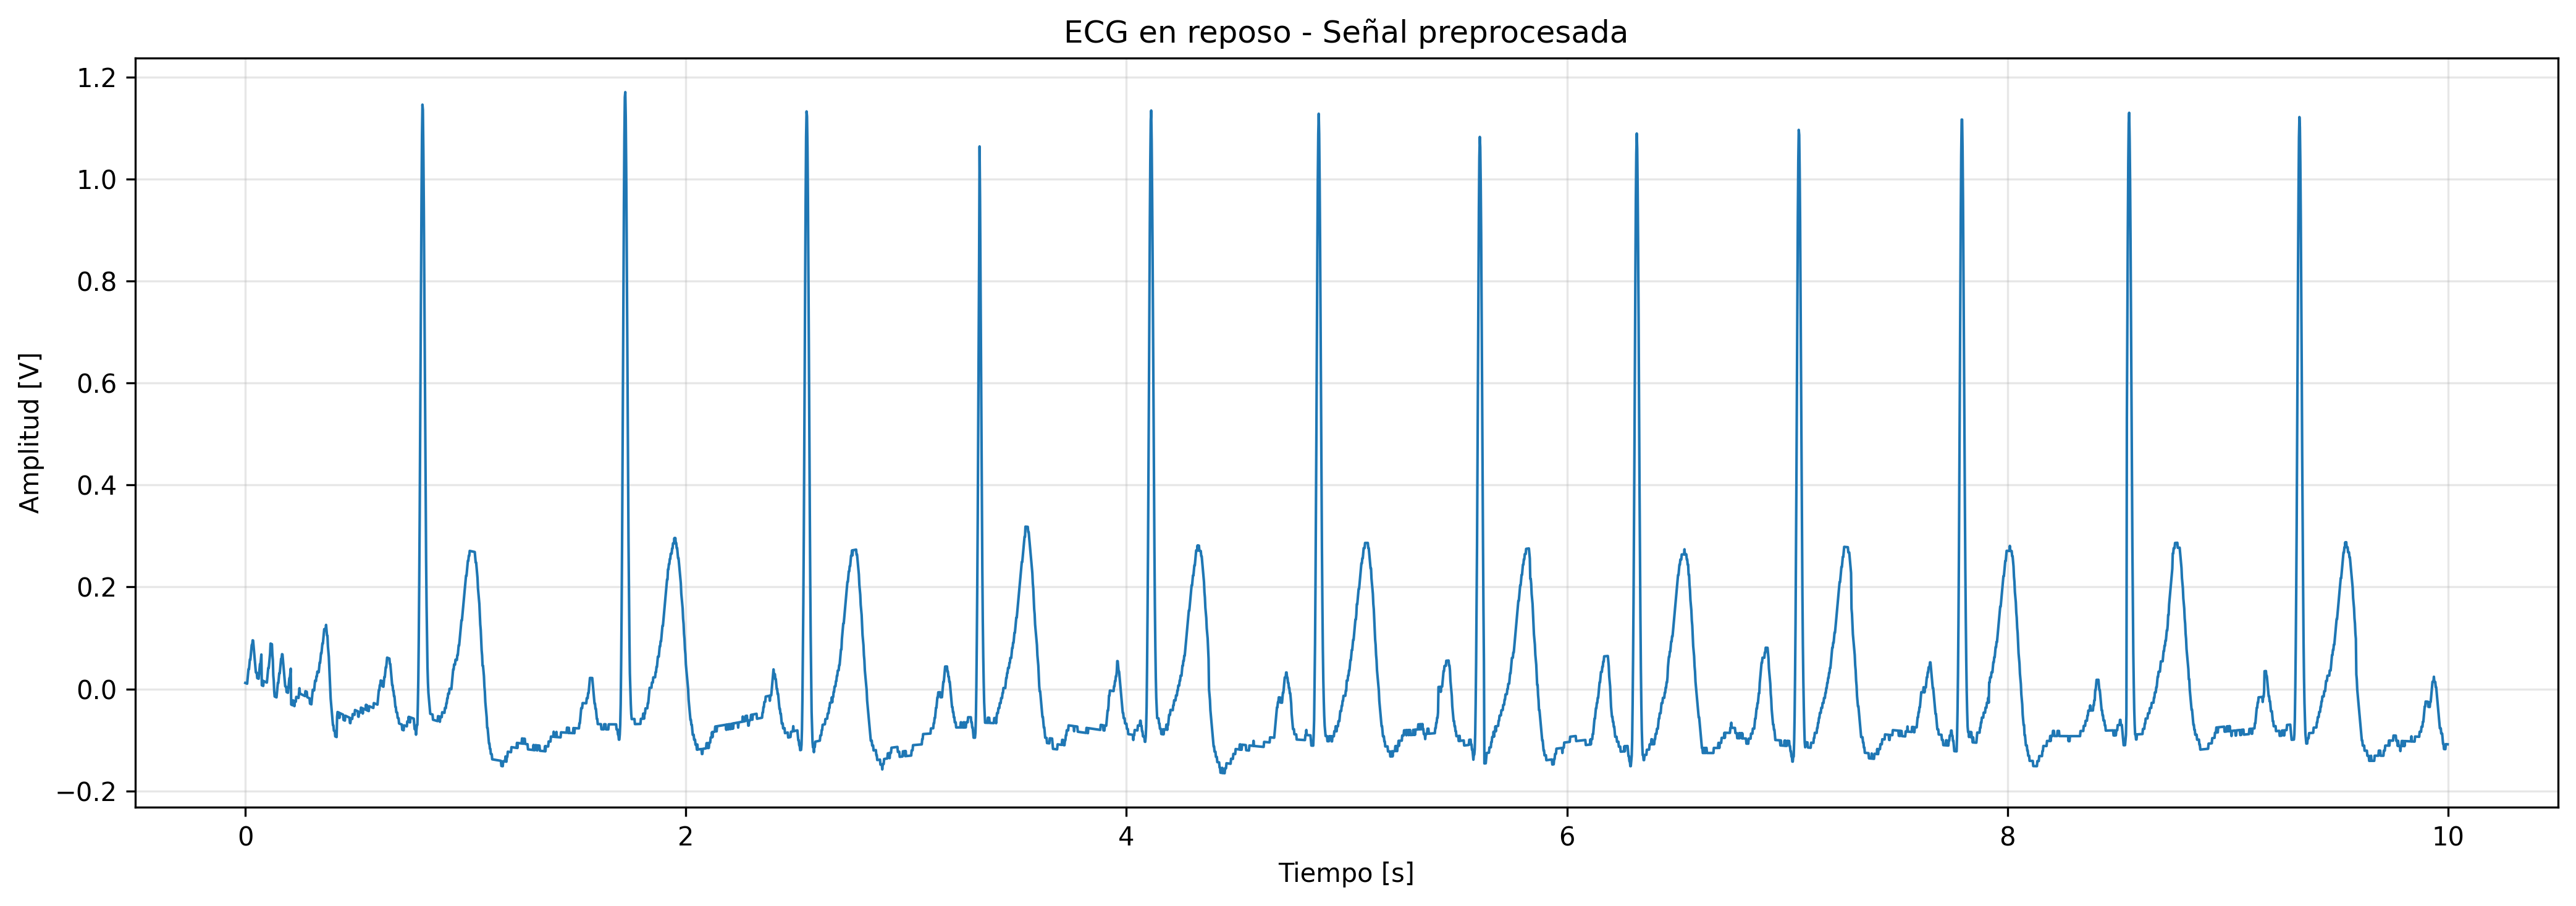
\includegraphics[width=0.95\textwidth]{Imagenes/ECG_Pre_Procesado_Zoom.png}
    \caption{Ventana ampliada de la señal de ECG preprocesada en reposo}
    \label{fig:procesado-pre-zoom}
\end{figure}

\begin{figure}[htbp]
    \centering
    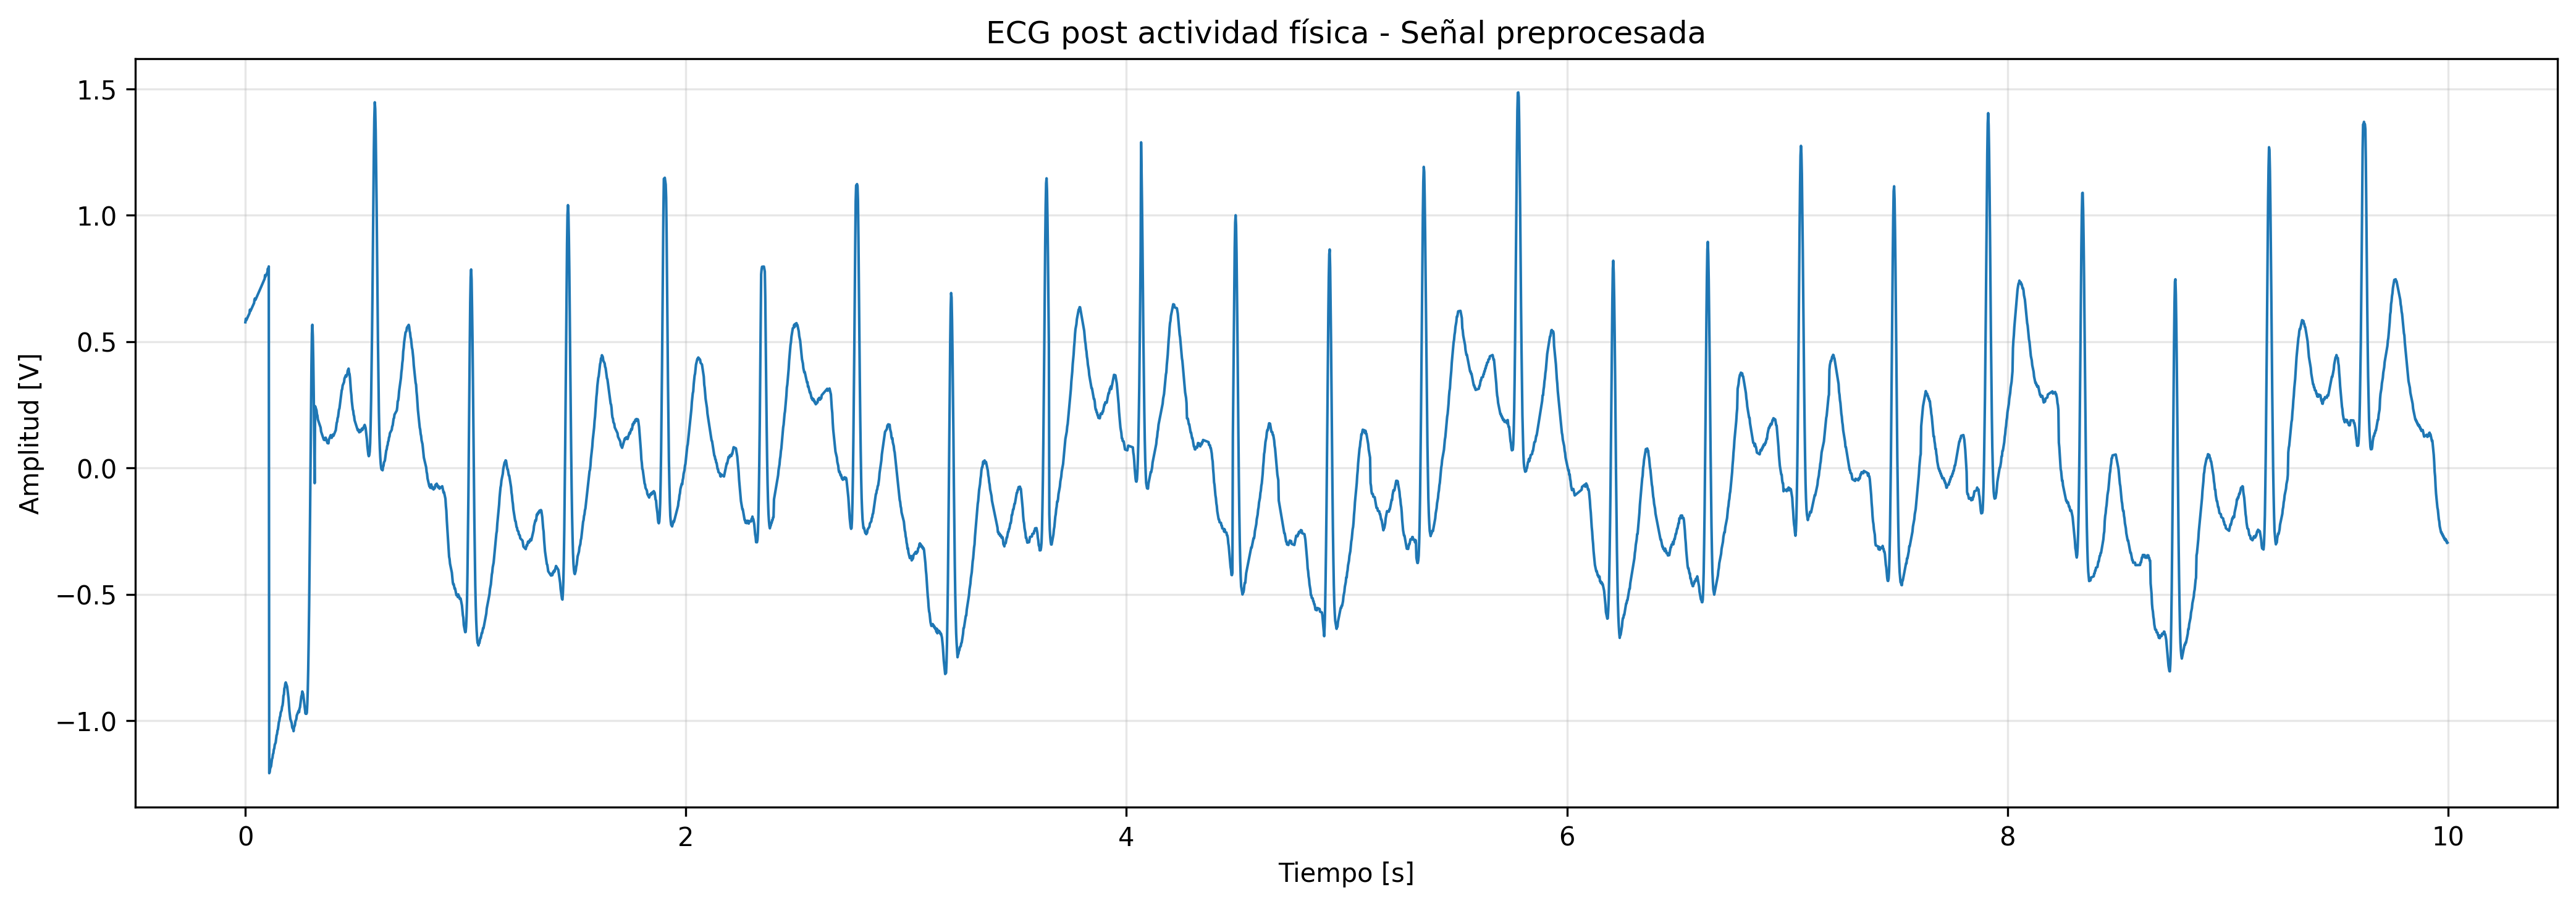
\includegraphics[width=0.95\textwidth]{Imagenes/ECG_Post_Procesado_Zoom.png}
    \caption{Ventana ampliada de la señal de ECG preprocesada luego de la actividad física}
    \label{fig:procesado-post-zoom}
\end{figure}

\FloatBarrier

Estas señales constituyen la entrada para la siguiente etapa del trabajo, en la
cual se realizará la detección automática de los complejos QRS mediante el
algoritmo de Pan--Tompkins.


% =========================
% BIBLIOGRAFÍA
% =========================

\clearpage
\section*{Bibliografía}
\addcontentsline{toc}{section}{Bibliografía}

% Sangría francesa de 1,27 cm, correspondiente al formato APA
\newcommand{\aparef}[1]{%
    \par
    \noindent
    \hangindent=1.27cm
    \hangafter=1
    #1
    \par
    \vspace{0.7em}
}

\aparef{
Analog Devices, Inc. (2020).
\textit{AD8232: Single-lead, heart rate monitor front end}
(Rev. D) [Hoja de datos].
}

\aparef{
Ashley, E. A., \& Niebauer, J. (2004).
\textit{Cardiology explained} (Cap. 3, Conquering the ECG).
Remedica.
}

\aparef{
DICOM Standards Committee. (2024).
\textit{DICOM PS3.3 2024b: Information object definitions---12-lead ECG IOD}.
National Electrical Manufacturers Association.
}

\aparef{
Kemp, B., Värri, A., Rosa, A. C., Nielsen, K. D., \& Gade, J. (1992).
A simple format for exchange of digitized polygraphic recordings.
\textit{Electroencephalography and Clinical Neurophysiology, 82}(5),
391--393.
doi: 10.1016/0013-4694(92)90009-7.
}

\aparef{
Moody, G. B. (2019).
\textit{WFDB Programmer's Guide}
(10th ed., revised for WFDB library version 10.6.2).
PhysioNet.
}

\aparef{
Noble, R. J., Hillis, J. S., \& Rothbaum, D. A. (1990).
Electrocardiography. En H. K. Walker, W. D. Hall, \& J. W. Hurst
(Eds.), \textit{Clinical methods: The history, physical, and laboratory
examinations} (3rd ed., Cap. 33). Butterworths.
}

\aparef{
U.S. Food and Drug Administration. (2021).
\textit{ECG waveform data: Frequently asked questions}.
}

\end{document}
